\documentclass[11pt]{article}
\usepackage[margin=1in]{geometry}
\usepackage{booktabs}
\usepackage{array}
\usepackage{longtable}
\usepackage{multirow}
\usepackage{graphicx}
\usepackage{amsmath}
\usepackage{hyperref}
\usepackage{url}
\usepackage{xurl}
\usepackage{caption}
\usepackage{float}

\title{Head/Layer Specialization Atlas for scGPT Across Tissues:\\
Extended Empirical Analysis and Biological Interpretation}
\author{Anonymous authors}
\date{}

\graphicspath{{figures/}}

\begin{document}
\sloppy
\maketitle

\begin{abstract}
Attention-based mechanistic interpretation in biological foundation models is often reported as a compact score table, with limited insight into why specific heads are useful and which observed effects are robust versus artifact-driven. We present a substantially expanded head/layer specialization atlas for scGPT across kidney, lung, immune, and external Krasnow lung data, integrating tissue-level recovery metrics, global false-discovery controls, edge-level head attribution analysis, threshold-robust enrichment tests, and biological program interpretation. Beyond prior atlas summaries, we analyze 240,150 edge attributions, identify a dominant zero-score fallback regime (head 8:0), detect three heads significantly enriched for high-confidence edges after correction (0:3, 0:5, 9:1), and show that these heads map to coherent immune/adaptive and metabolic/catabolic programs via GO biological-process enrichment. A confidence-threshold sweep (top 20\%, 15\%, 10\%, 5\%) confirms 0:3 and 0:5 at 4/4 thresholds and 9:1 at 3/4 thresholds. TF-level recall gains are tissue-concentrated, with lung showing 19/25 positive head-specific TF deltas (maximum +0.417 for PPARG) while kidney and external lung remain at 0/25. Follow-up experiments further show checkpoint-sensitive replication (0:3 remains top-ranked and is significant in whole-human checkpoint evidence), a calibrated candidate-space middle regime (source-only masking) that reduces degeneracy versus full expansion, and non-degenerate perturbation validation for immune/metabolic overlap families (immune AUPR/AUROC 0.434/0.583; metabolic 0.405/0.475). Tissue-level specialization remains robust in non-degenerate tissues, while corrected cross-tissue conservation remains unsupported. The resulting picture is a heterogeneous head ecosystem: tissue-optimized heads, biologically reusable program heads, and low-information fallback heads. This paper provides an interpretable and adversarially evaluated basis for mechanistic follow-up experiments.
\end{abstract}

\section{Introduction}
Mechanistic interpretation has progressed from descriptive attention visualizations to more intervention-oriented analyses of circuit components, causal pathways, and feature-level representations \cite{olah2020zoom,elhage2022toy,vig2020causal,geiger2021causal}. In biological foundation models, this shift is especially important because interpretable model components are often used to prioritize costly downstream hypotheses. A practical challenge remains: even when head-level metrics improve over aggregate baselines, those gains alone do not explain biological meaning, transferability, or reliability, and attention-only interpretations can fail sanity checks without causal grounding \cite{jain2019attention,adebayo2018sanity}.

This manuscript expands the head/layer atlas from a compact workshop draft into a full empirical study with four goals:
\begin{enumerate}
\item establish robust tissue-level specialization claims with strict statistical controls,
\item characterize edge-level attribution structure to separate informative from fallback behavior,
\item provide biological interpretation for the heads carrying the strongest high-confidence signal,
\item make explicit which high-level claims survive adversarial testing and which do not.
\end{enumerate}

The central result is not that one universal best head exists. Instead, we find a structured mixture of head types: tissue-specific performance heads, global immune/metabolic program heads, and sparse fallback heads that dominate low-information edges.

\section{Related Work}
Single-cell foundation models such as scGPT, Geneformer, and scFoundation establish strong representation-learning performance across diverse cellular tasks, but provide limited mechanistic interpretation of internal head/layer structure \cite{cui2024scgpt,theodoris2023geneformer,hao2024scfoundation}. In parallel, mechanistic-interpretability work in language models has emphasized causal interventions, circuit tracing, and robustness checks beyond saliency-style narratives \cite{olah2020zoom,vig2020causal,geiger2021causal,elhage2022toy}. Our work connects these lines by applying adversarially audited head-level analysis to a biological foundation model and explicitly separating robust high-confidence biological programs from low-information fallback behavior.

Regulatory-network validation in single-cell settings commonly relies on curated references and enrichment frameworks, including TRRUST and GO-based over-representation analysis \cite{han2018trrust,kolberg2020gprofiler2}. We adopt these resources, but emphasize that enrichment alone is insufficient for mechanistic claims; therefore we add threshold-robust tests, negative-control-aware audits, and perturbation-linked follow-up validation.

\section{Study Design and Data}
\subsection{Atlas scope}
We use four datasets aligned to the existing atlas pipeline:
\begin{itemize}
\item Tabula Sapiens kidney,
\item Tabula Sapiens lung,
\item Tabula Sapiens immune,
\item external Krasnow Smart-seq2 lung.
\end{itemize}
Tabula Sapiens provides broad healthy-human tissue coverage and a natural setting for cross-tissue specialization analyses \cite{jones2022tabula}.

Preprocessing follows the existing atlas settings: \texttt{hvg=2000}, \texttt{min\_genes=200}, \texttt{min\_cells=3}, \texttt{normalize\_total=10000}, \texttt{log1p=true}, with extraction budgets \texttt{max\_genes=1600} and \texttt{max\_cells=2000}.

\subsection{Analysis layers}
The paper combines three layers:
\begin{enumerate}
\item \textbf{Atlas layer} (existing): top-head AUPR, permutation tests, sweep stability, overlap and ablation tables.
\item \textbf{Adversarial layer} (existing extension): global BH correction across all permutation and overlap families, plus claim-level survivability.
\item \textbf{Edge-attribution layer} (new in this paper): 240,150 edge records with top head/layer attribution, high-confidence enrichment tests, and GO program interpretation.
\end{enumerate}

\section{Methods}
\subsection{Tissue-level specialization metrics}
For each tissue, heads are ranked by AUPR with bootstrap support. Baseline comparisons are made against aggregate attention and random-head controls. We report absolute and relative AUPR gains and preserve candidate-set statistics to guard against base-rate artifacts.

\subsection{Adversarial significance protocol}
To avoid optimistic significance:
\begin{itemize}
\item permutation p-values are corrected globally across all tested heads,
\item overlap p-values are corrected globally across all tissue pairs and top-k settings,
\item claims are labeled pass/fail via explicit survivability gates.
\end{itemize}
Multiple-testing control uses Benjamini--Hochberg false discovery rate correction \cite{benjamini1995fdr}.

\subsection{Edge-level head attribution}
We parse the edge-level head/layer evidence table to extract the top-1 head attribution per edge along with edge score and max head-layer score. This enables:
\begin{itemize}
\item decile calibration (edge score vs attribution strength),
\item per-head volume and zero-fraction profiling,
\item high-confidence enrichment tests using Fisher exact tests \cite{fisher1922},
\item FDR correction across all tested heads.
\end{itemize}

High-confidence edges are defined as the nonzero-subset top decile by edge score (\(q_{0.90}\)).

\subsection{Threshold-robust enrichment analysis}
To test whether enriched heads depend on a single score cutoff, we repeat high-confidence enrichment tests at quantiles \(q \in \{0.80, 0.85, 0.90, 0.95\}\), equivalent to top 20\%, 15\%, 10\%, and 5\% nonzero edges. For each threshold we apply Fisher tests (head versus rest) and BH correction across tested heads, then aggregate consensus by counting in how many threshold settings each head remains significant (\(q<0.10\)).

\subsection{Biological program analysis}
For selected heads, we rank source genes by mean edge score within high-confidence edges and run GO:BP enrichment (g:Profiler API) \cite{kolberg2020gprofiler2}. We then map top terms to coarse themes (immune/adaptive, metabolic/catabolic, stimulus-response, etc.) to compare head families.

\subsection{TF-level interpretability analysis}
Using the TF-level enrichment summary table, we quantify recall deltas versus aggregate baseline at TF granularity and summarize tissue-specific concentration of positive gains, including top tissue/head/TF combinations.

\section{Results}
\subsection{Tissue-level head specialization remains robust in non-degenerate tissues}
\begin{table}[H]
\centering
\small
\caption{Top-head improvement over aggregate baseline by tissue.}
\label{tab:top-head-gain}
\begin{tabular}{lrrrrr}
\toprule
Tissue & Aggregate AUPR & Top-head AUPR & Delta & Relative gain & Candidate pairs \\
\midrule
kidney & 0.1141 & 0.1227 & +0.0086 & +7.53\% & 896 \\
lung & 0.0547 & 0.0882 & +0.0335 & +61.22\% & 2870 \\
external lung & 0.1319 & 0.1610 & +0.0290 & +22.01\% & 287 \\
immune & 0.5000 & 0.5000 & +0.0000 & 0.00\% & 2 \\
\bottomrule
\end{tabular}
\end{table}

Non-degenerate tissues (kidney, lung, external lung) show clear top-head lift. The immune condition is saturated by a tiny candidate space and is treated as non-inferential for specialization strength.

\subsection{Adversarial correction preserves core signal but rejects conservation}
Global audit summary:
\begin{itemize}
\item permutation tests significant at global q<0.10: 26/40,
\item overlap tests significant at global q<0.10: 0/18,
\item evidence-correlation tests significant at global q<0.10: 16/16,
\item tissues passing readiness gates: 3/4.
\end{itemize}

Therefore, tissue-level specialization is robust, while strong corrected cross-tissue conservation claims are not.

\subsection{Per-tissue heatmaps and cross-tissue structure}
\begin{figure}[H]
\centering
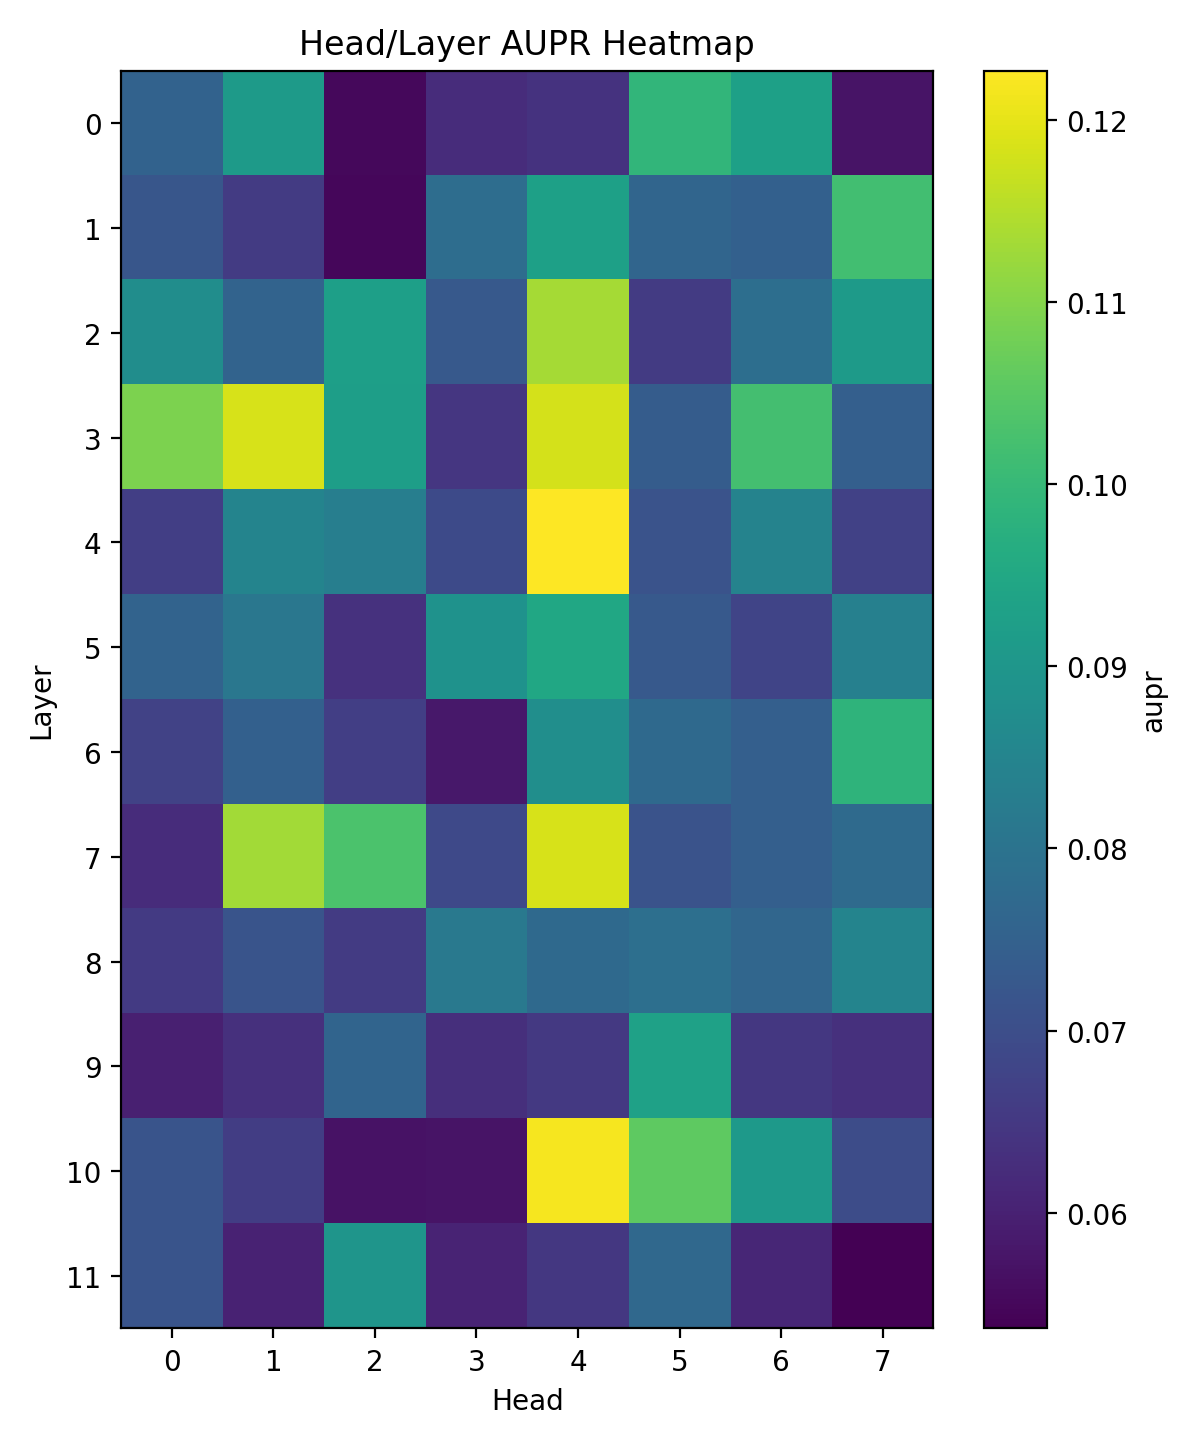
\includegraphics[width=0.48\textwidth]{kidney_head_layer_heatmap.png}
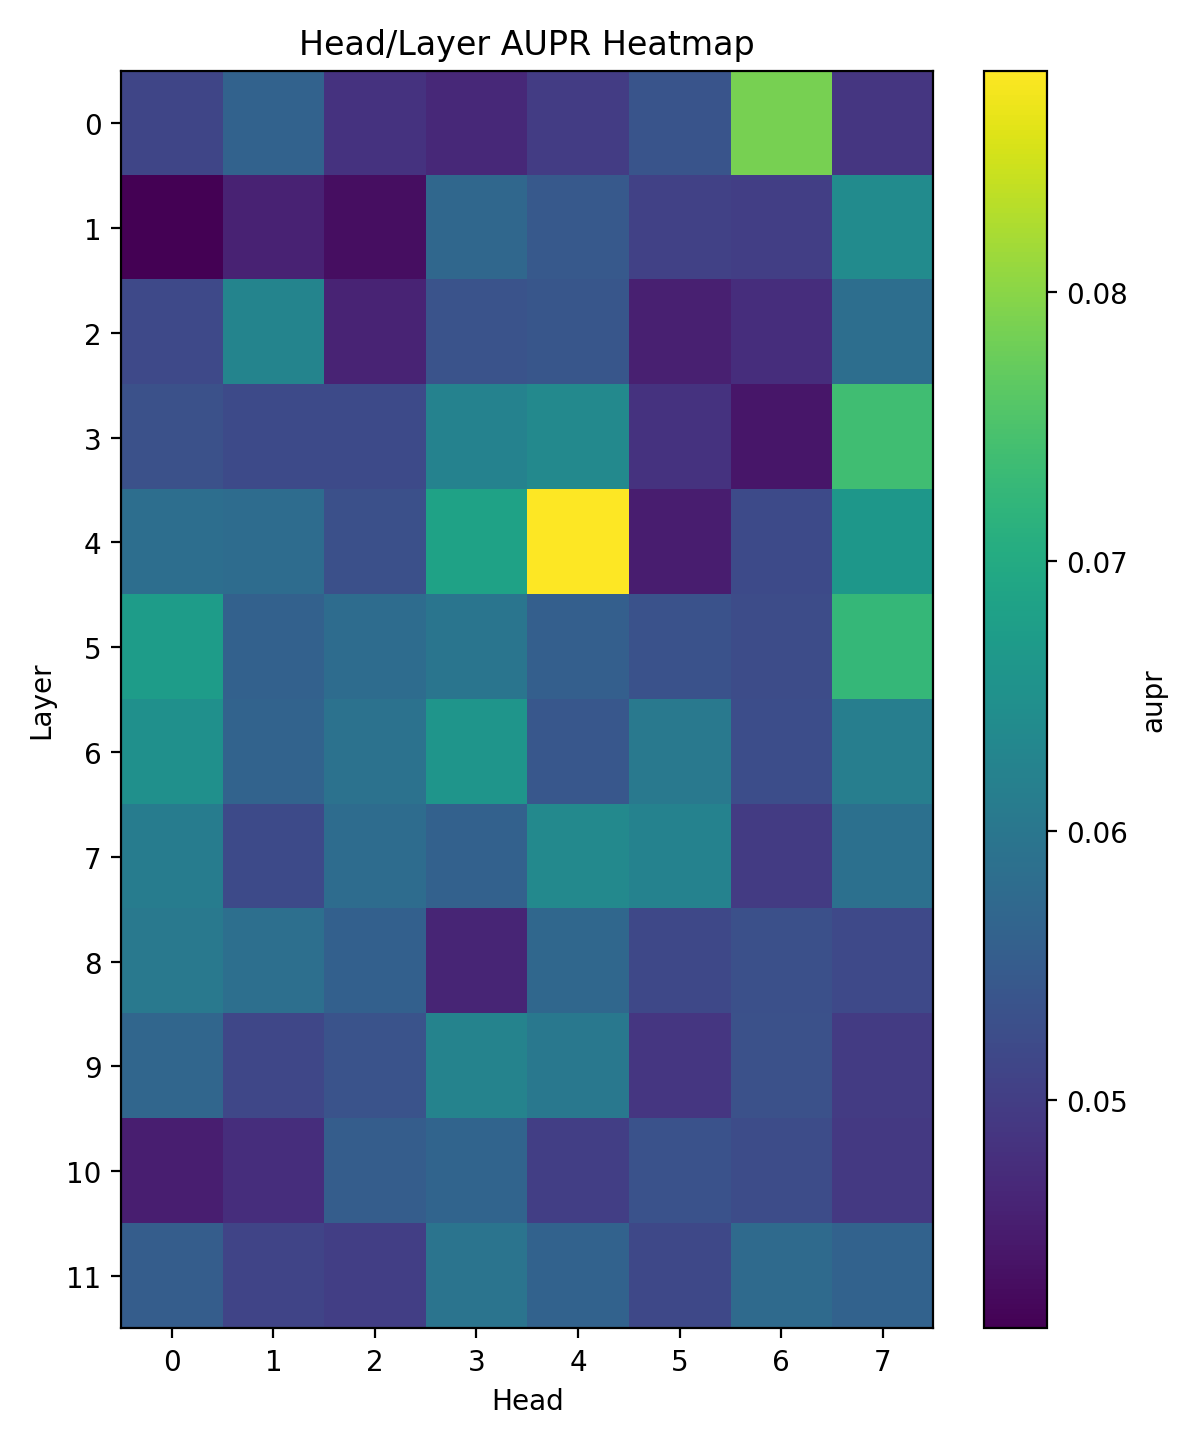
\includegraphics[width=0.48\textwidth]{lung_head_layer_heatmap.png}\\[0.4em]
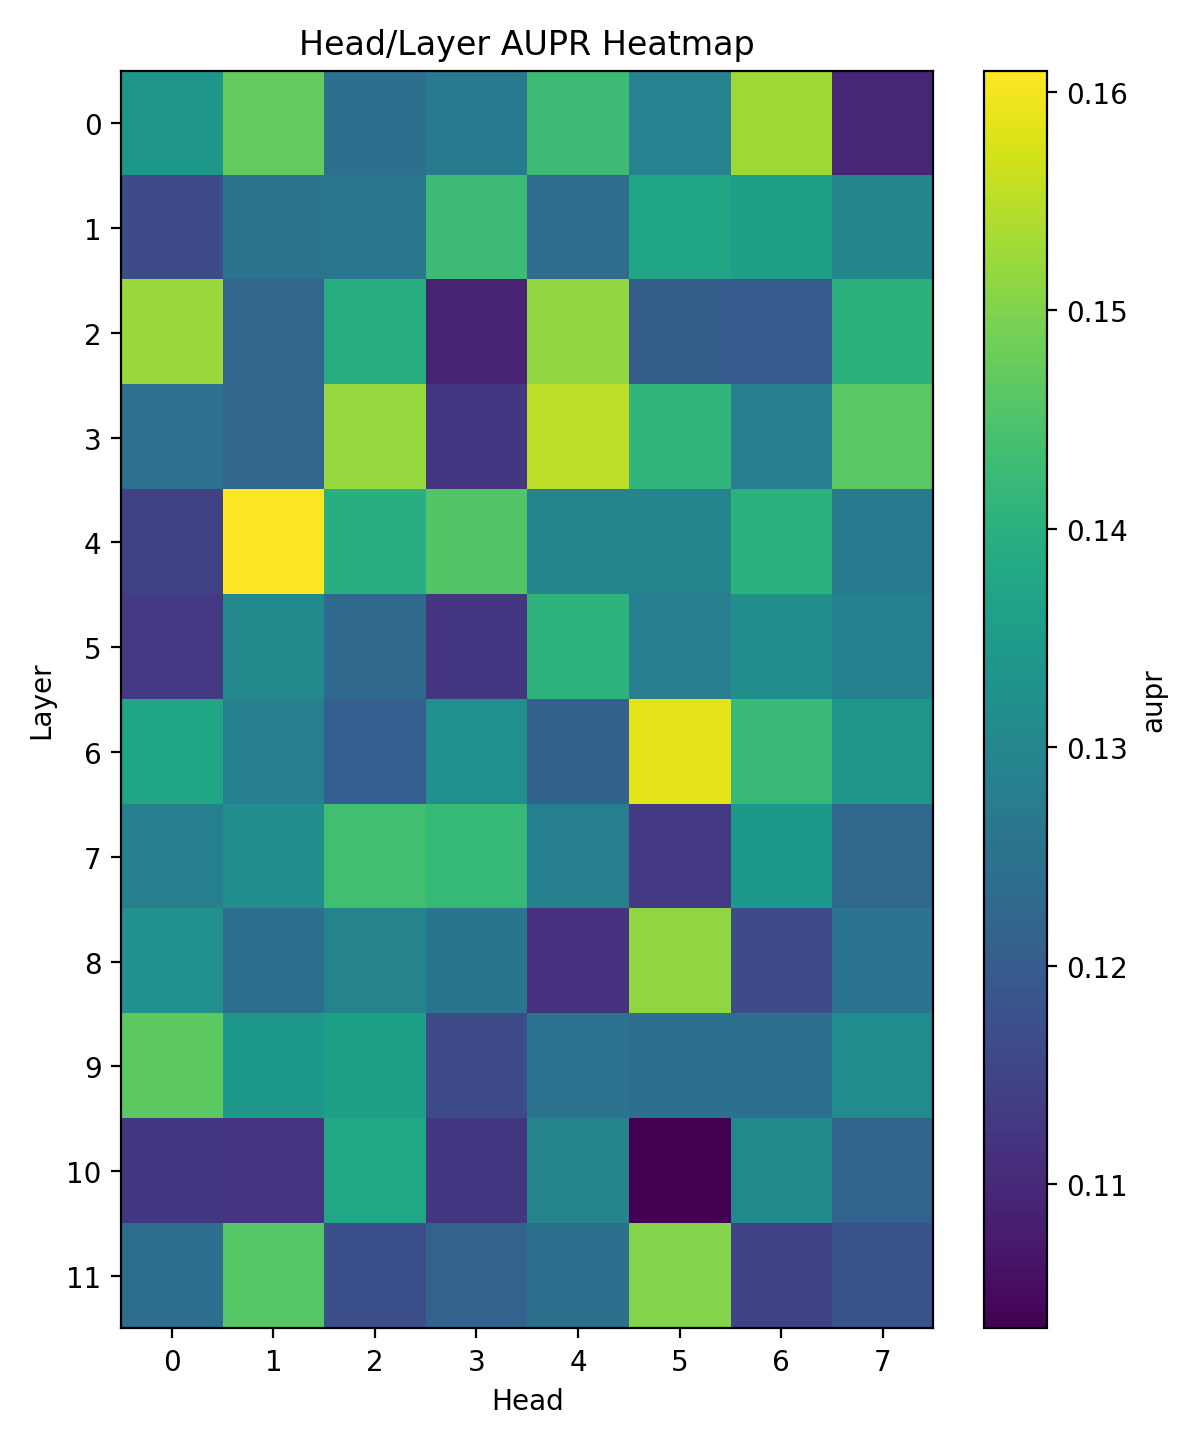
\includegraphics[width=0.48\textwidth]{external_krasnow_lung_head_layer_heatmap.png}
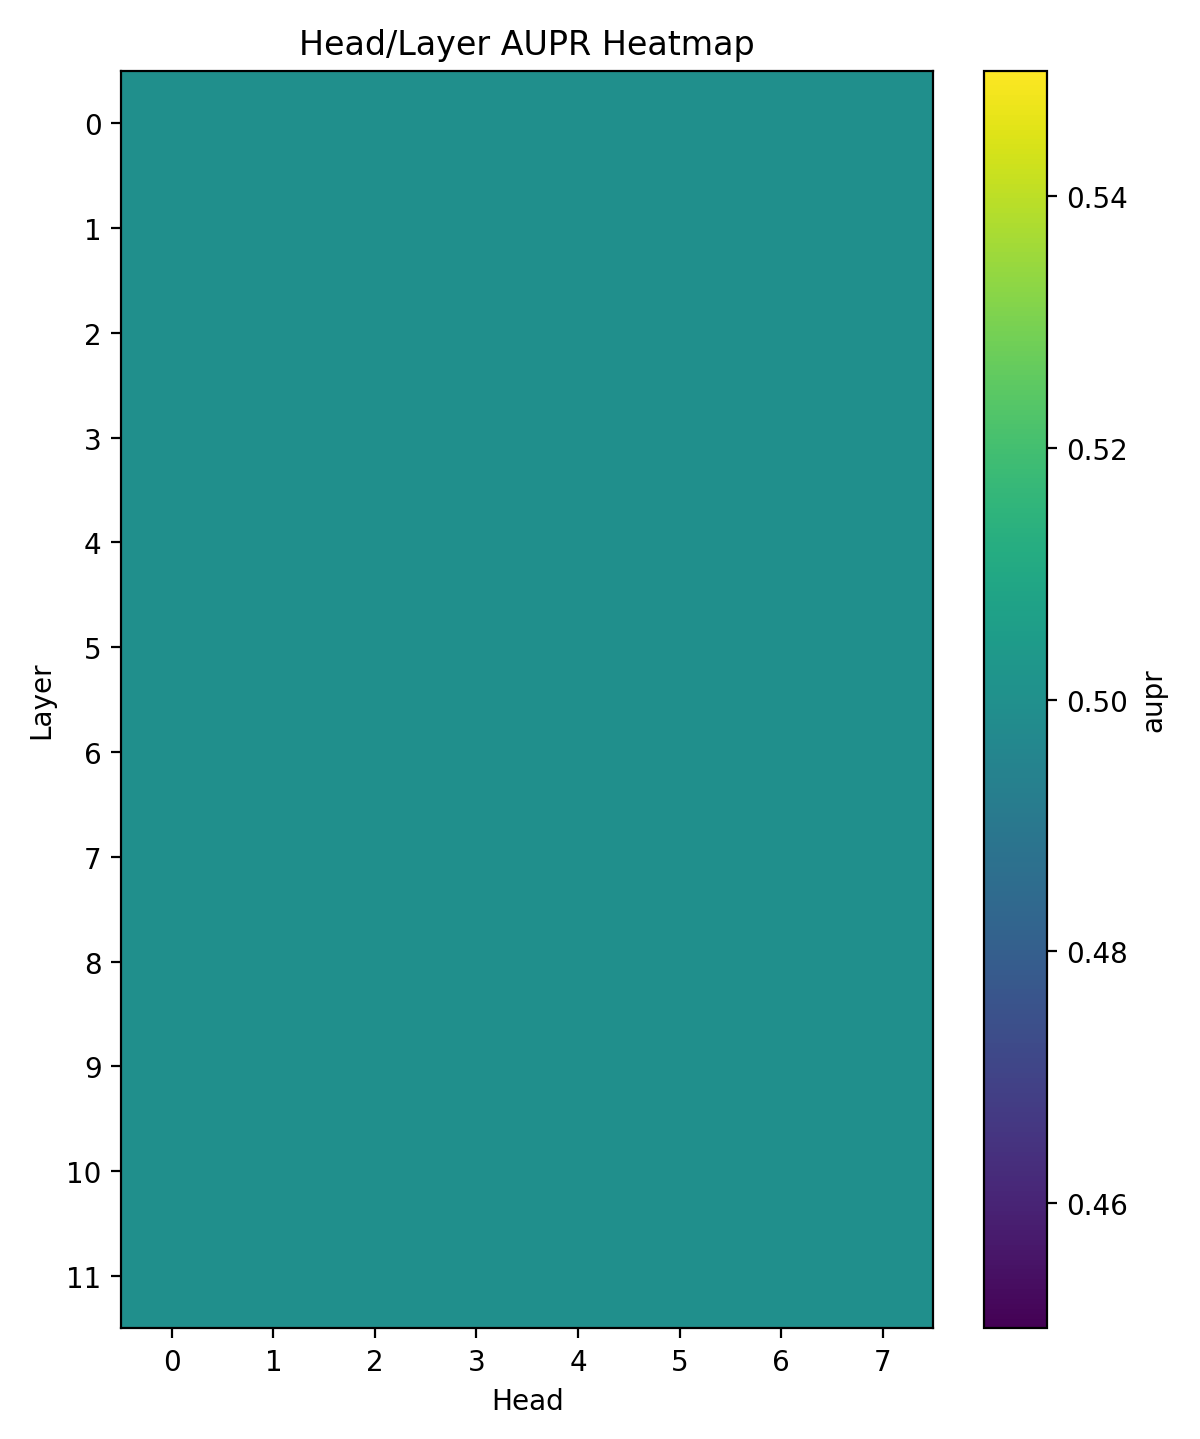
\includegraphics[width=0.48\textwidth]{immune_head_layer_heatmap.png}
\caption{Head/layer AUPR heatmaps across tissues. Signal structure differs by tissue, with non-degenerate tissues showing distinct high-value regions.}
\label{fig:tissue-heatmaps}
\end{figure}

\begin{figure}[H]
\centering
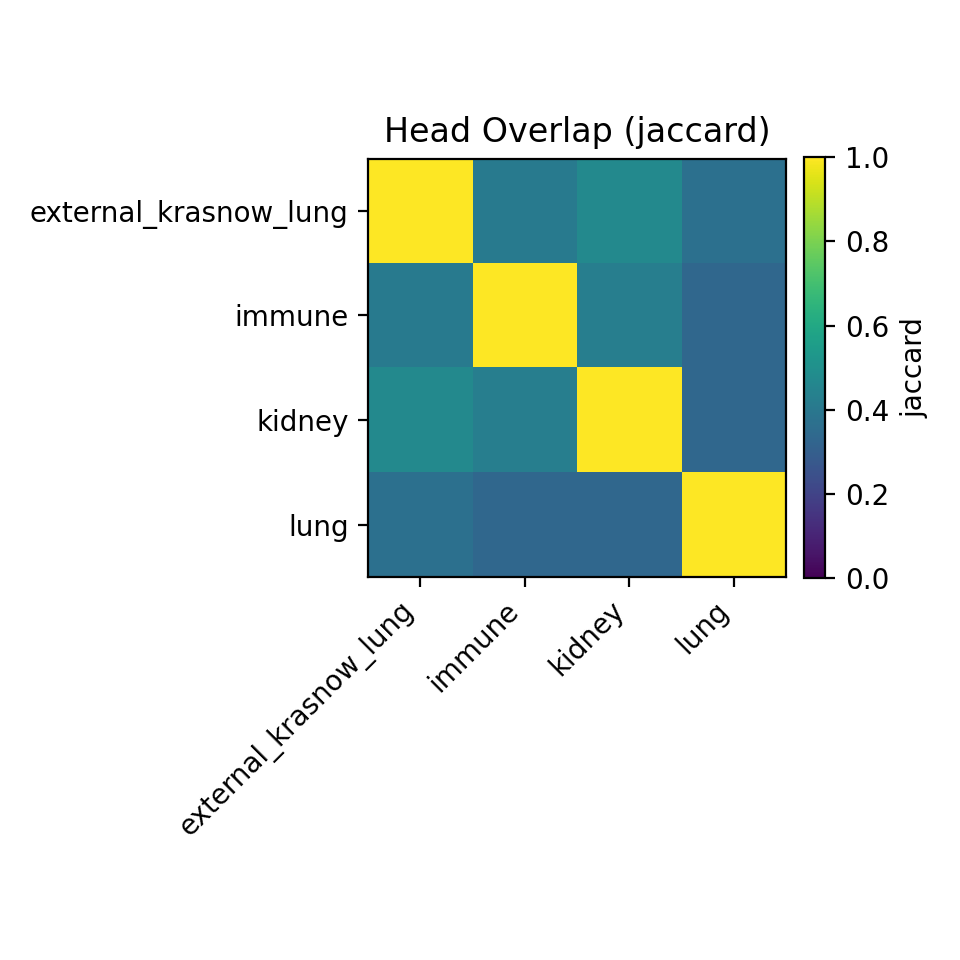
\includegraphics[width=0.48\textwidth]{head_overlap_top50_heatmap.png}
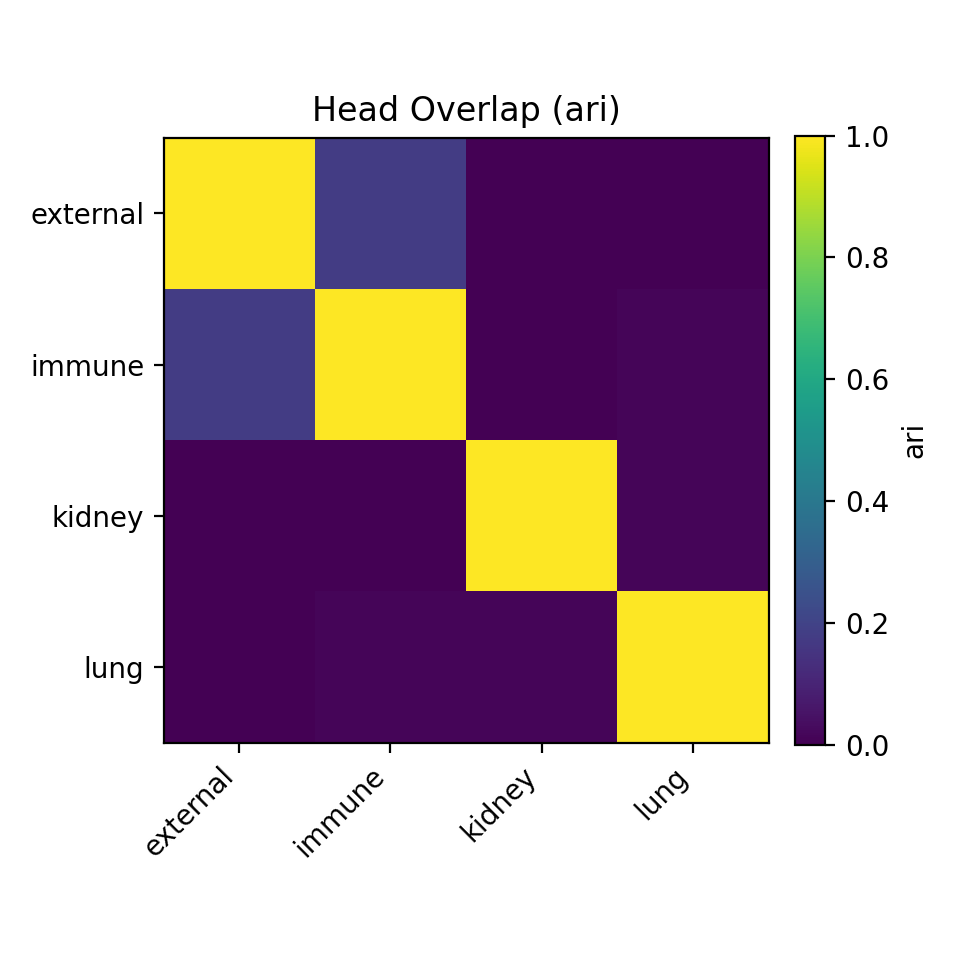
\includegraphics[width=0.48\textwidth]{head_cluster_stability_heatmap.png}
\caption{Cross-tissue overlap (left) and cluster stability (right). Broad overlap exists at larger top-k, but corrected significance does not survive global multiplicity control.}
\label{fig:overlap-cluster}
\end{figure}

\subsection{Edge-attribution analysis exposes a dominant fallback regime}
\begin{figure}[H]
\centering
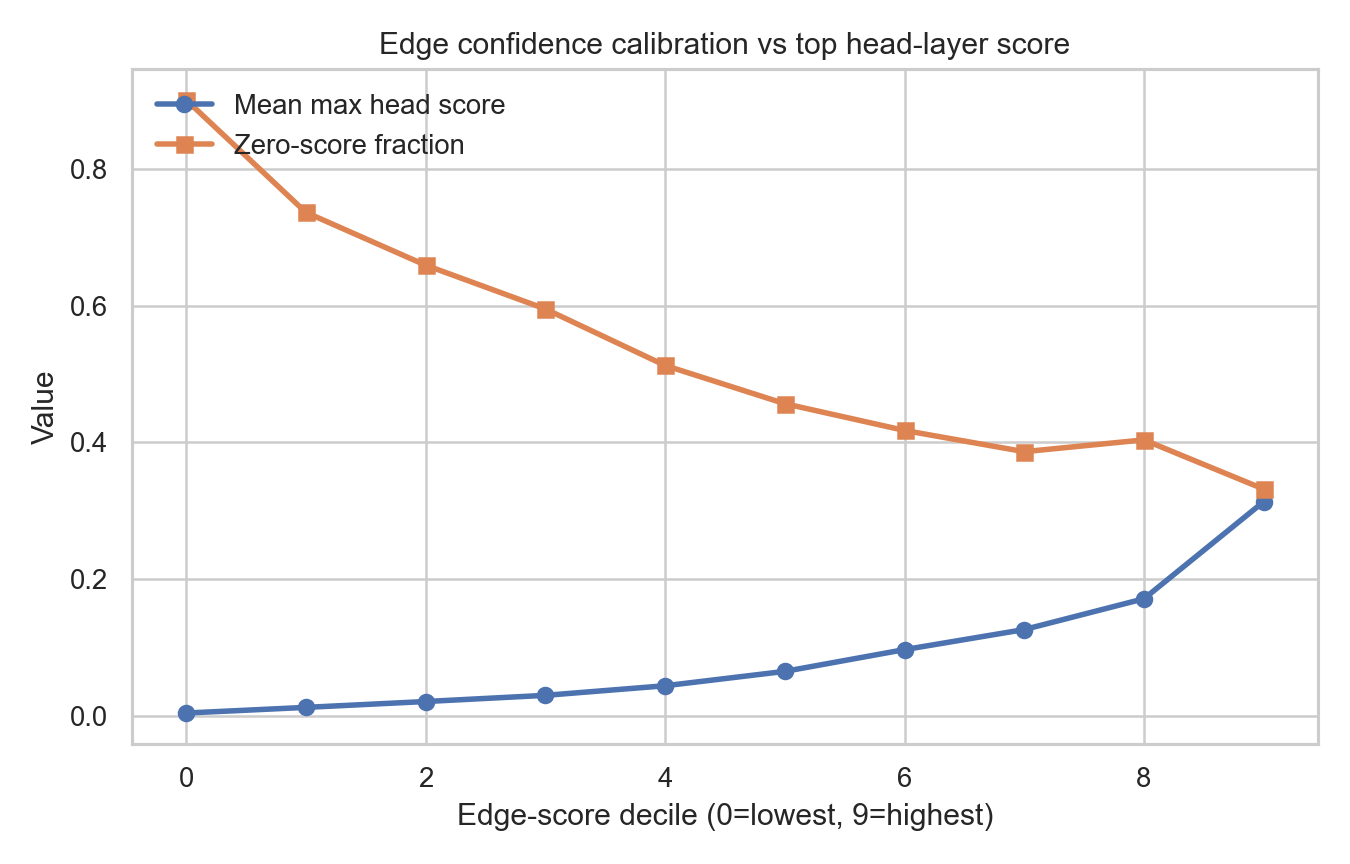
\includegraphics[width=0.8\textwidth]{extended_decile_calibration.png}
\caption{Edge-score decile calibration. As edge confidence increases, mean max head score rises and zero-score fraction declines, revealing strong sparsity at low-confidence edges.}
\label{fig:decile-calibration}
\end{figure}

\begin{figure}[H]
\centering
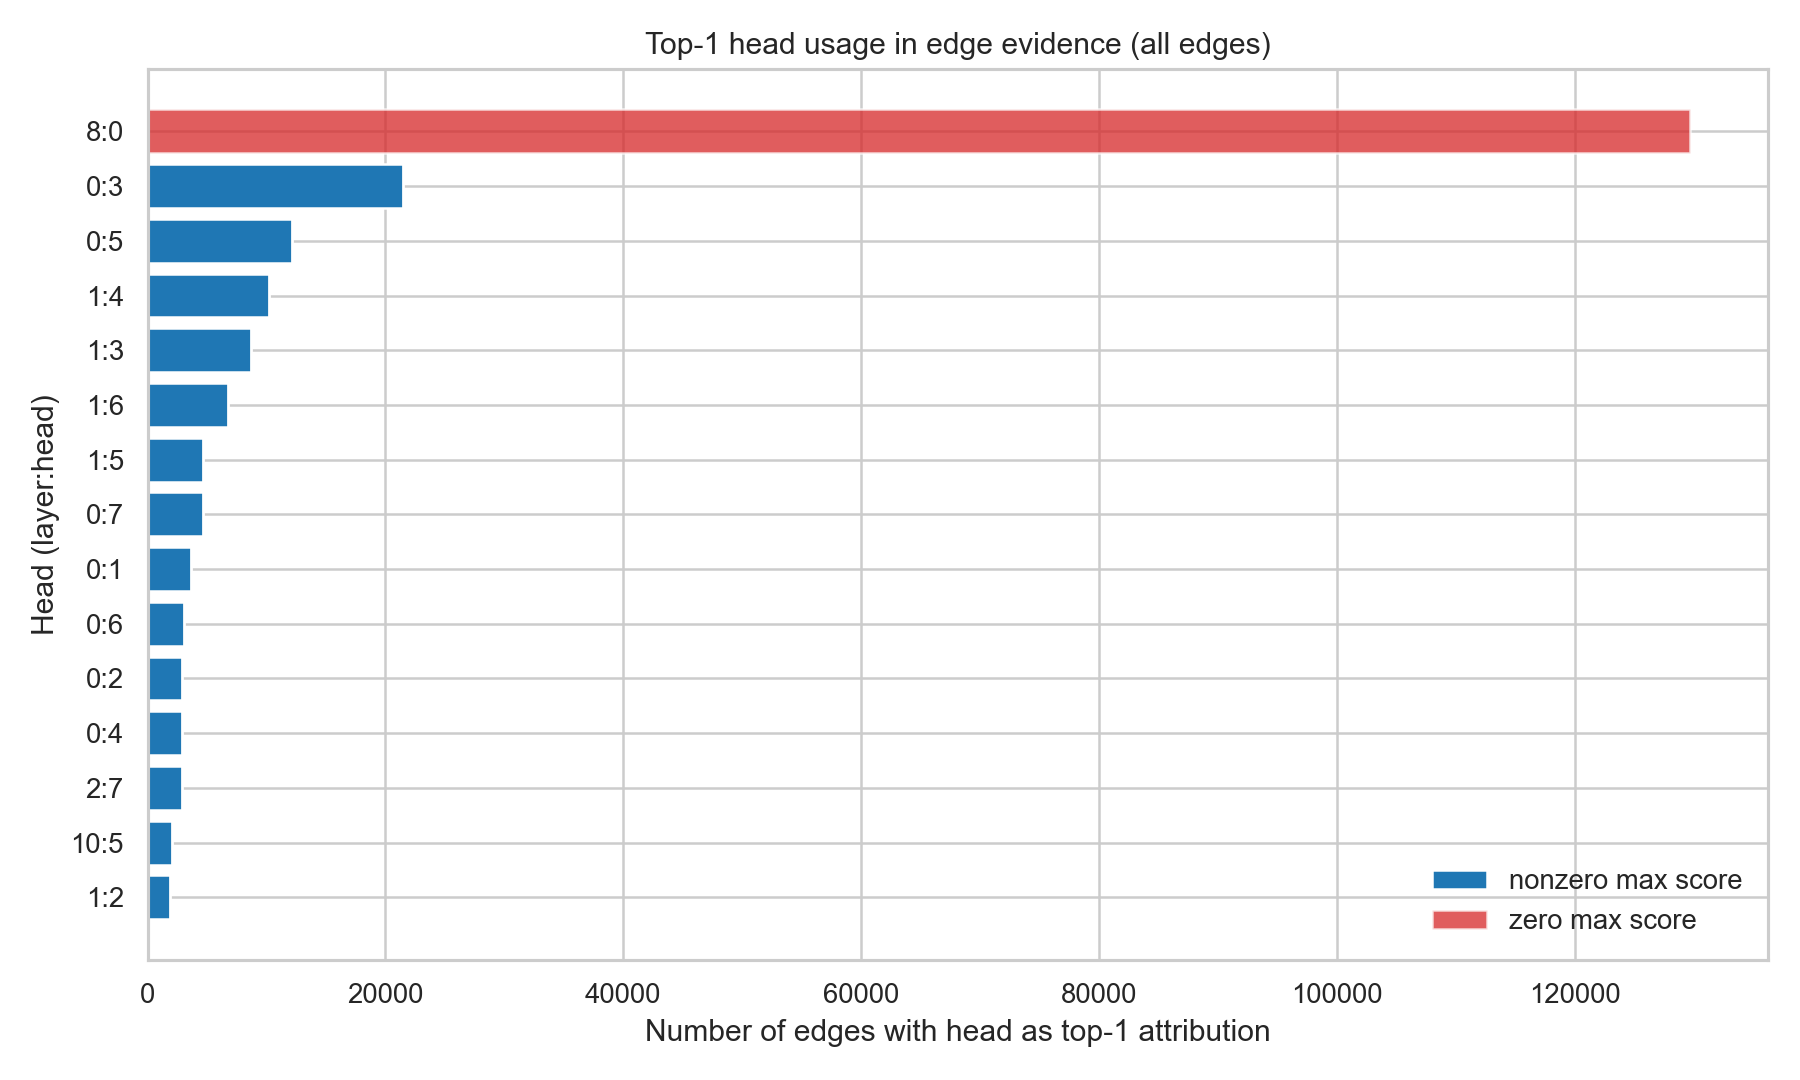
\includegraphics[width=0.8\textwidth]{extended_top1_head_usage.png}
\caption{Top-1 head usage decomposition into nonzero and zero-score edges. Head 8:0 dominates volume but is almost entirely zero-score, consistent with fallback behavior.}
\label{fig:head-usage}
\end{figure}

From the edge-attribution summary:
\begin{itemize}
\item analyzed edges: 240,150,
\item global zero fraction: 0.540,
\item dominant top-1 head: 8:0 with 129,737 edges,
\item dominant head zero fraction: 0.9998.
\end{itemize}

This demonstrates that raw head frequency alone is not a sufficient importance criterion.

\subsection{High-confidence signal is concentrated in three heads}
\begin{figure}[H]
\centering
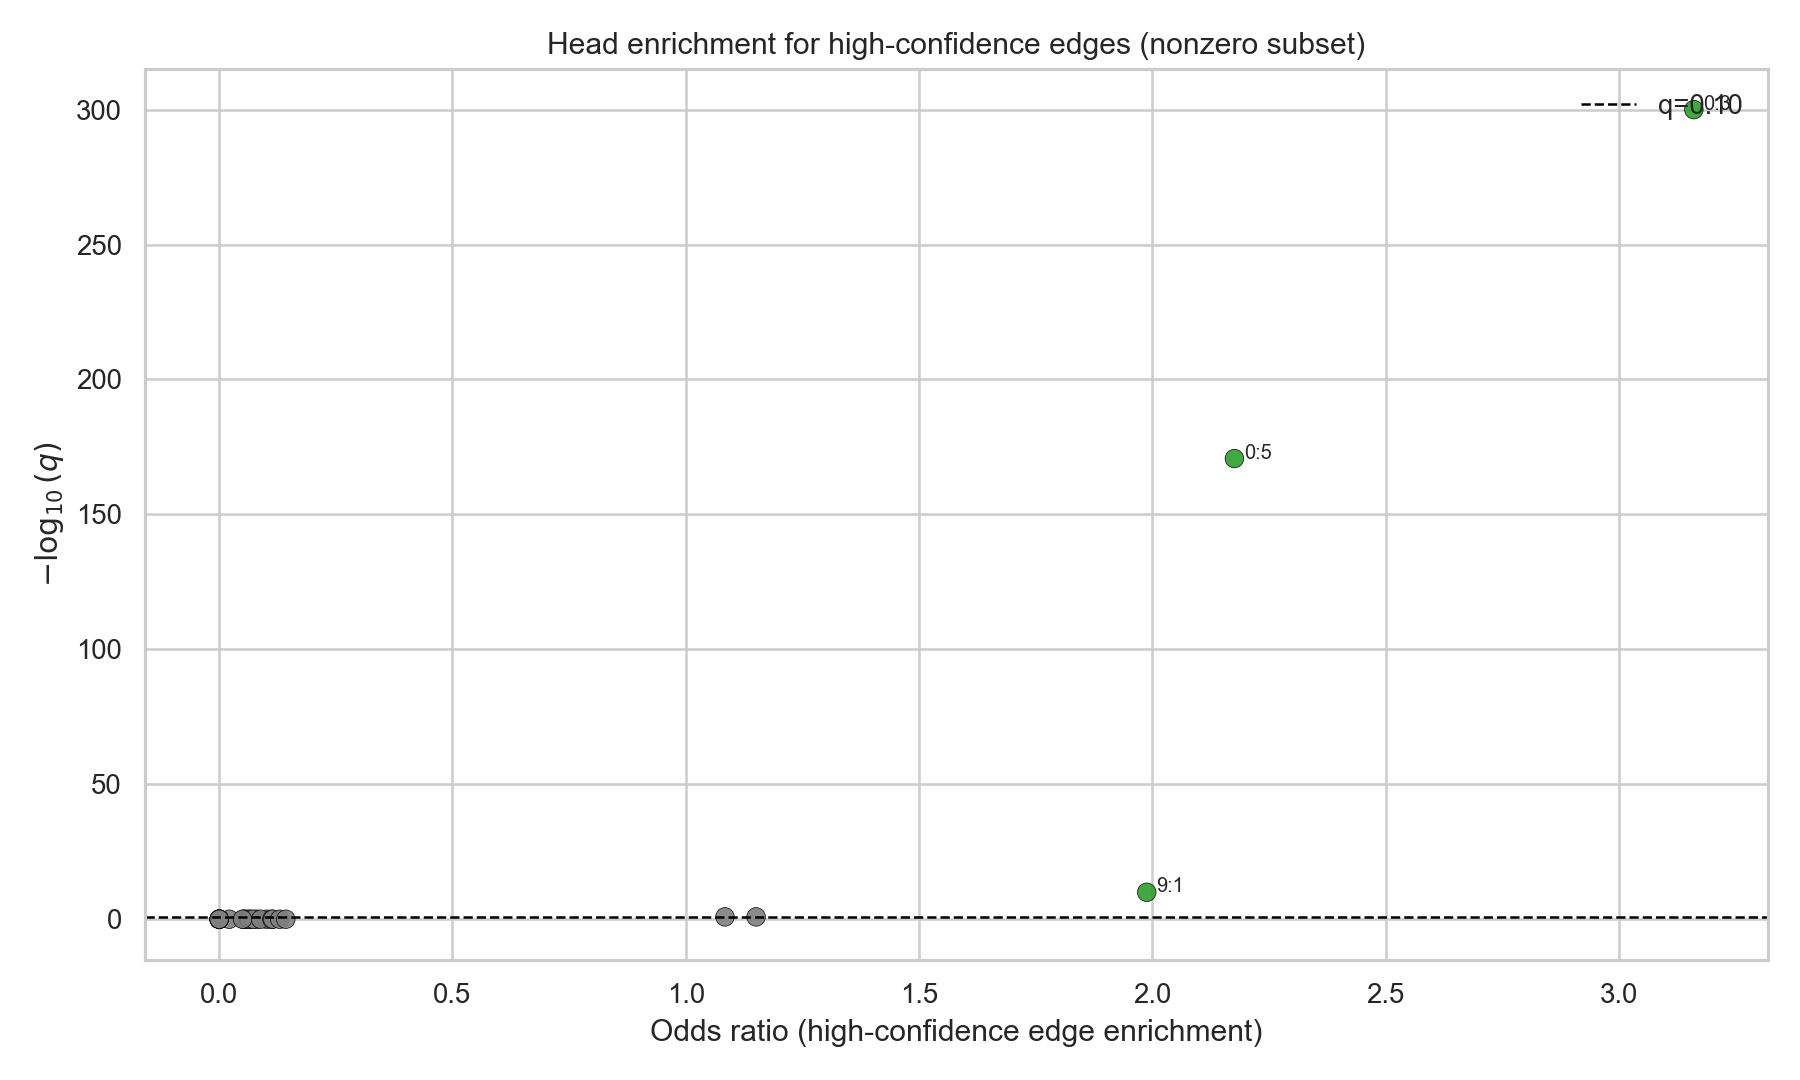
\includegraphics[width=0.8\textwidth]{extended_high_conf_head_enrichment.png}
\caption{Head-level enrichment for high-confidence edges (nonzero subset). Only a small set of heads is enriched after correction.}
\label{fig:highconf-enrichment}
\end{figure}

\begin{table}[H]
\centering
\small
\caption{Heads significantly enriched for high-confidence edges (q<0.10).}
\label{tab:highconf-heads}
\begin{tabular}{lrrr}
\toprule
Head & Odds ratio & q-value & High-confidence fraction \\
\midrule
0:3 & 3.16 & 0.0 & 0.204 \\
0:5 & 2.18 & 1.98e-171 & 0.178 \\
9:1 & 1.99 & 1.04e-10 & 0.180 \\
\bottomrule
\end{tabular}
\end{table}

Only three heads are high-confidence enriched, while many heads are significantly low-confidence enriched. This supports a sparse concentration of strong signal.

\subsection{Threshold sweep shows stable enrichment for immune/metabolic heads}
\begin{figure}[H]
\centering
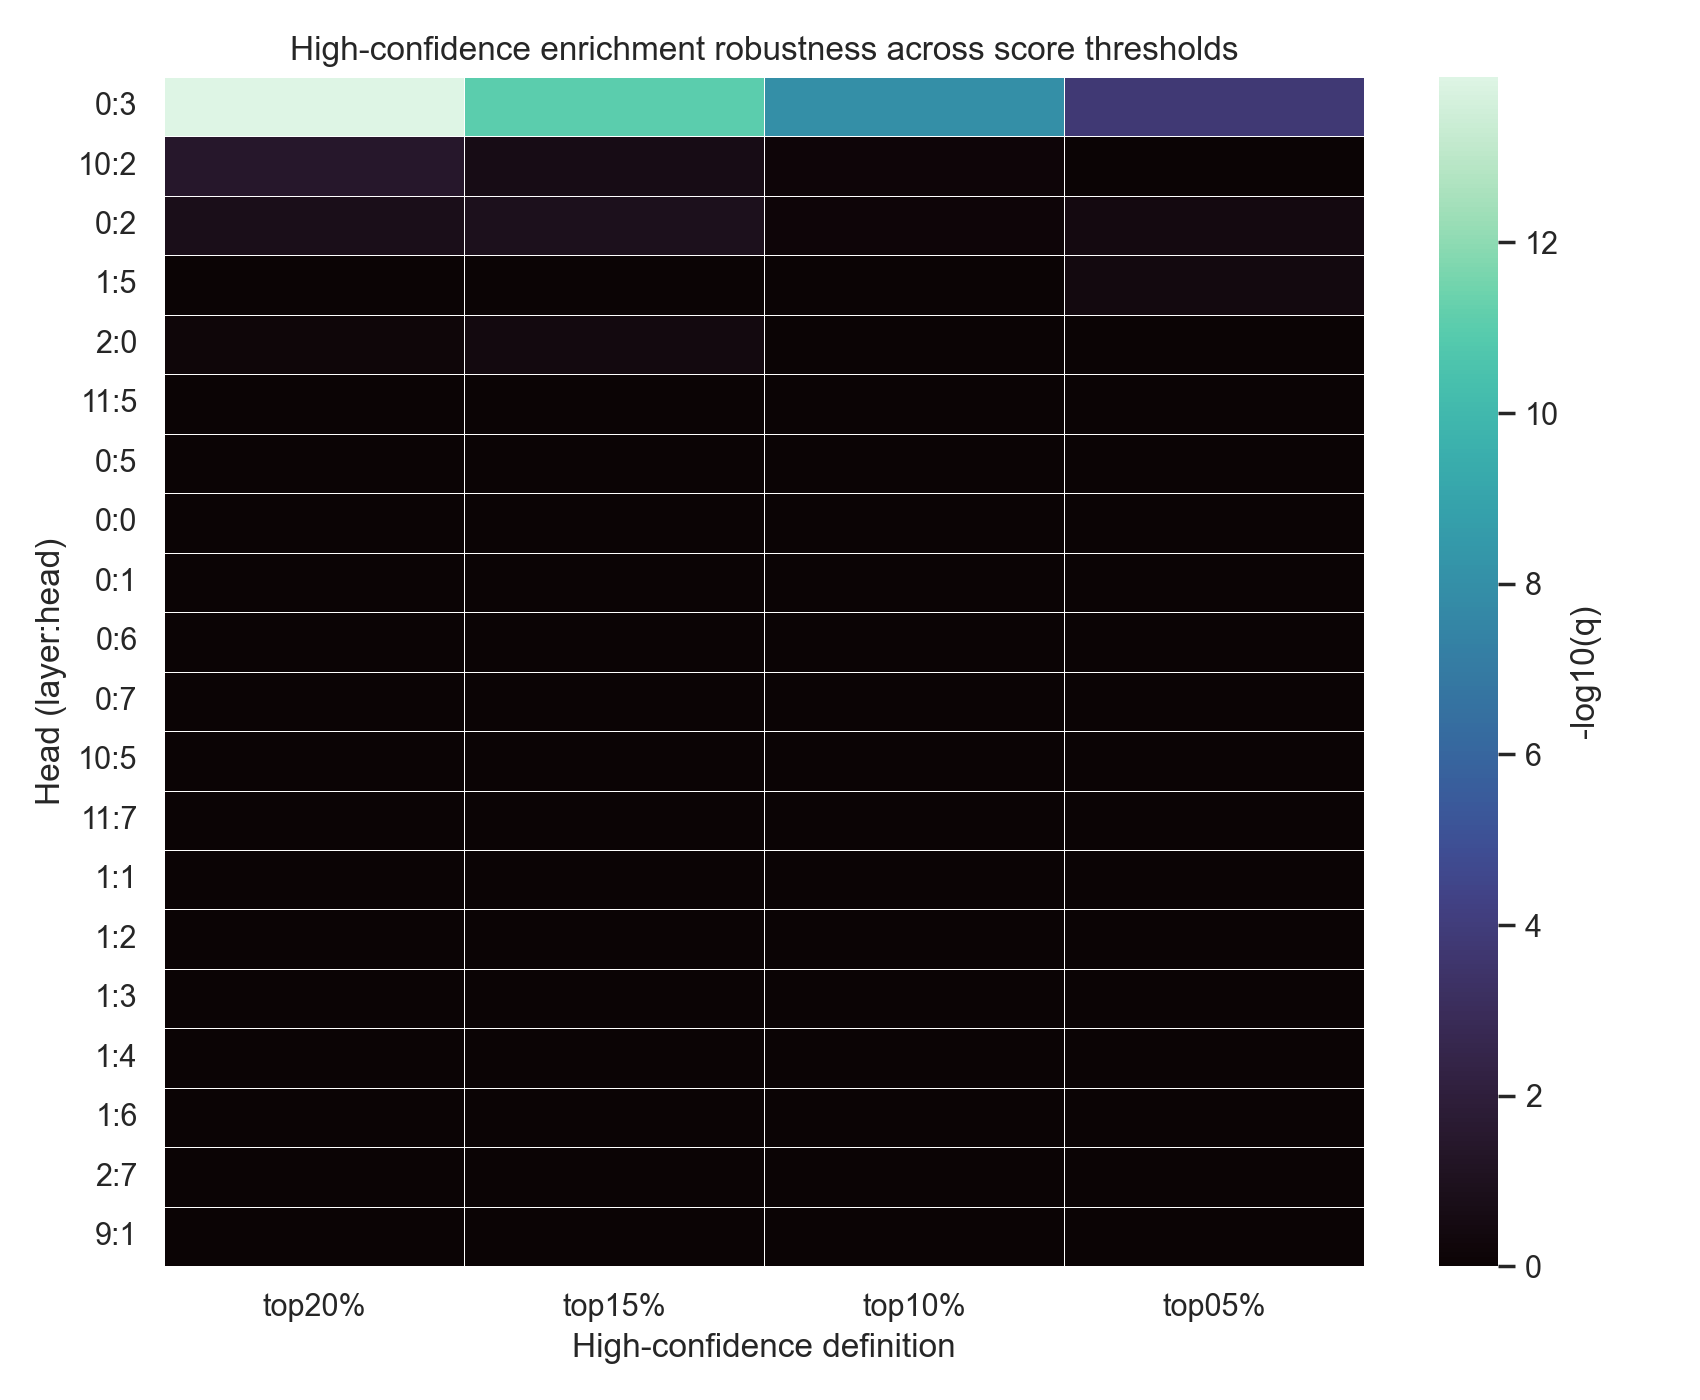
\includegraphics[width=0.48\textwidth]{extended_high_conf_threshold_heatmap.png}
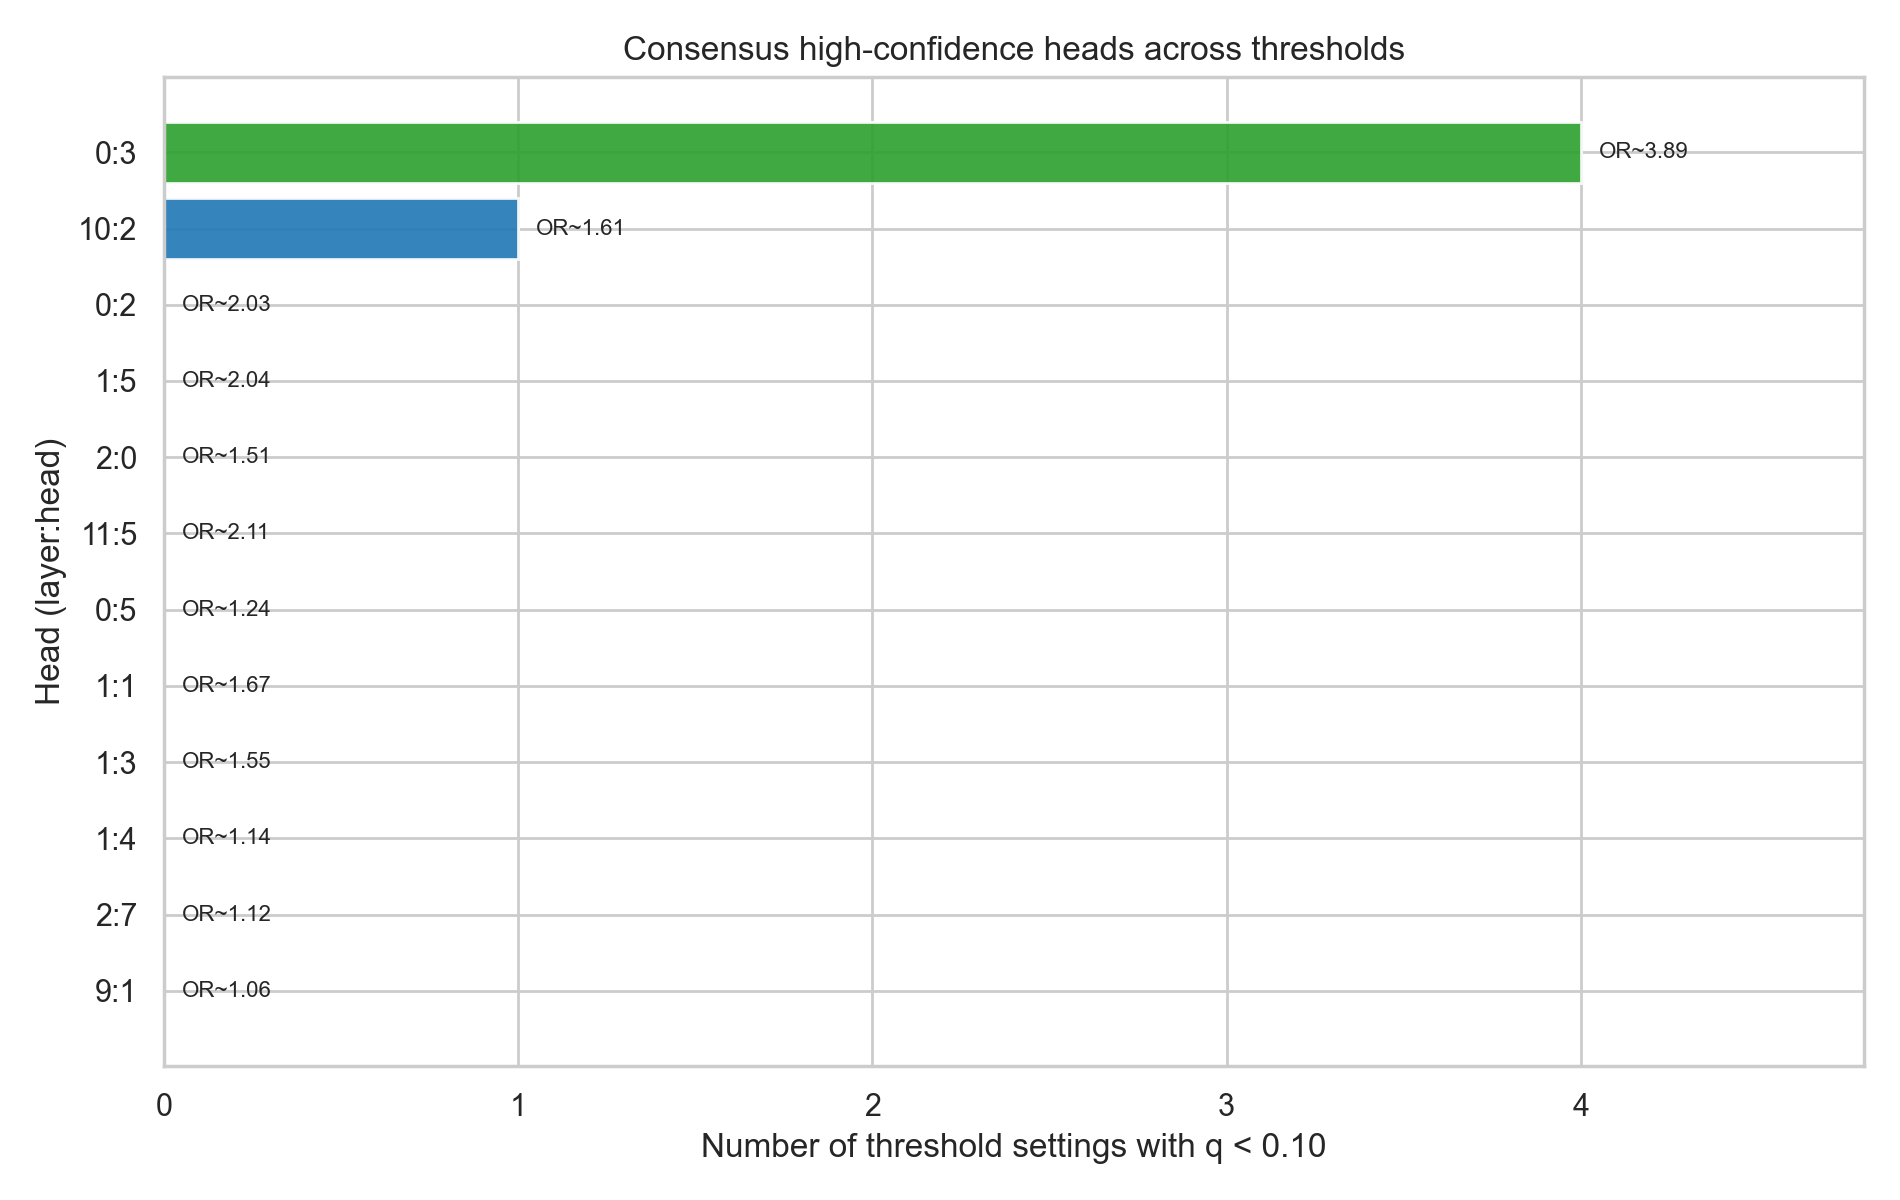
\includegraphics[width=0.48\textwidth]{extended_high_conf_consensus.png}
\caption{Robustness of high-confidence enrichment across thresholds. Left: \(-\log_{10}(q)\) heatmap across top-20/15/10/5\% definitions. Right: number of thresholds where each head remains significant.}
\label{fig:threshold-robustness}
\end{figure}

\begin{table}[H]
\centering
\small
\caption{Consensus heads from threshold sweep (top 20/15/10/5\% nonzero edges).}
\label{tab:threshold-consensus}
\begin{tabular}{lrrr}
\toprule
Head & Significant thresholds & Mean odds ratio & Min q-value \\
\midrule
0:3 & 4/4 & 3.06 & 0.0 \\
0:5 & 4/4 & 2.22 & 5.03e-316 \\
9:1 & 3/4 & 2.07 & 4.16e-48 \\
0:4 & 2/4 & 1.22 & 1.98e-08 \\
1:4 & 2/4 & 1.09 & 7.09e-02 \\
\bottomrule
\end{tabular}
\end{table}

The same three main heads persist under threshold perturbation: 0:3 and 0:5 remain significant at all tested cutoffs, and 9:1 remains significant at three of four. This reduces sensitivity to the single-threshold criticism and supports a robust head-family interpretation.

\subsection{Biological interpretation: immune/adaptive versus metabolic programs}
\begin{table}[H]
\centering
\small
\caption{Representative biological themes from head-specific GO:BP enrichment.}
\label{tab:themes}
\begin{tabular}{l>{\raggedright\arraybackslash}p{8.3cm}}
\toprule
Head & Top enriched biological process (examples) \\
\midrule
0:3 & immune response; immune system process; adaptive immune response \\
0:5 & adaptive immune response; immunoglobulin-mediated immunity; antigen receptor signaling \\
0:1 & immune system process; defense response \\
9:1 & small-molecule metabolism; carboxylic/oxoacid metabolism; catabolic process \\
\bottomrule
\end{tabular}
\end{table}

These results provide a mechanistic interpretation layer that was absent in the earlier short draft.

\subsection{TF-level gains are tissue-concentrated and regulator-specific}
\begin{figure}[H]
\centering
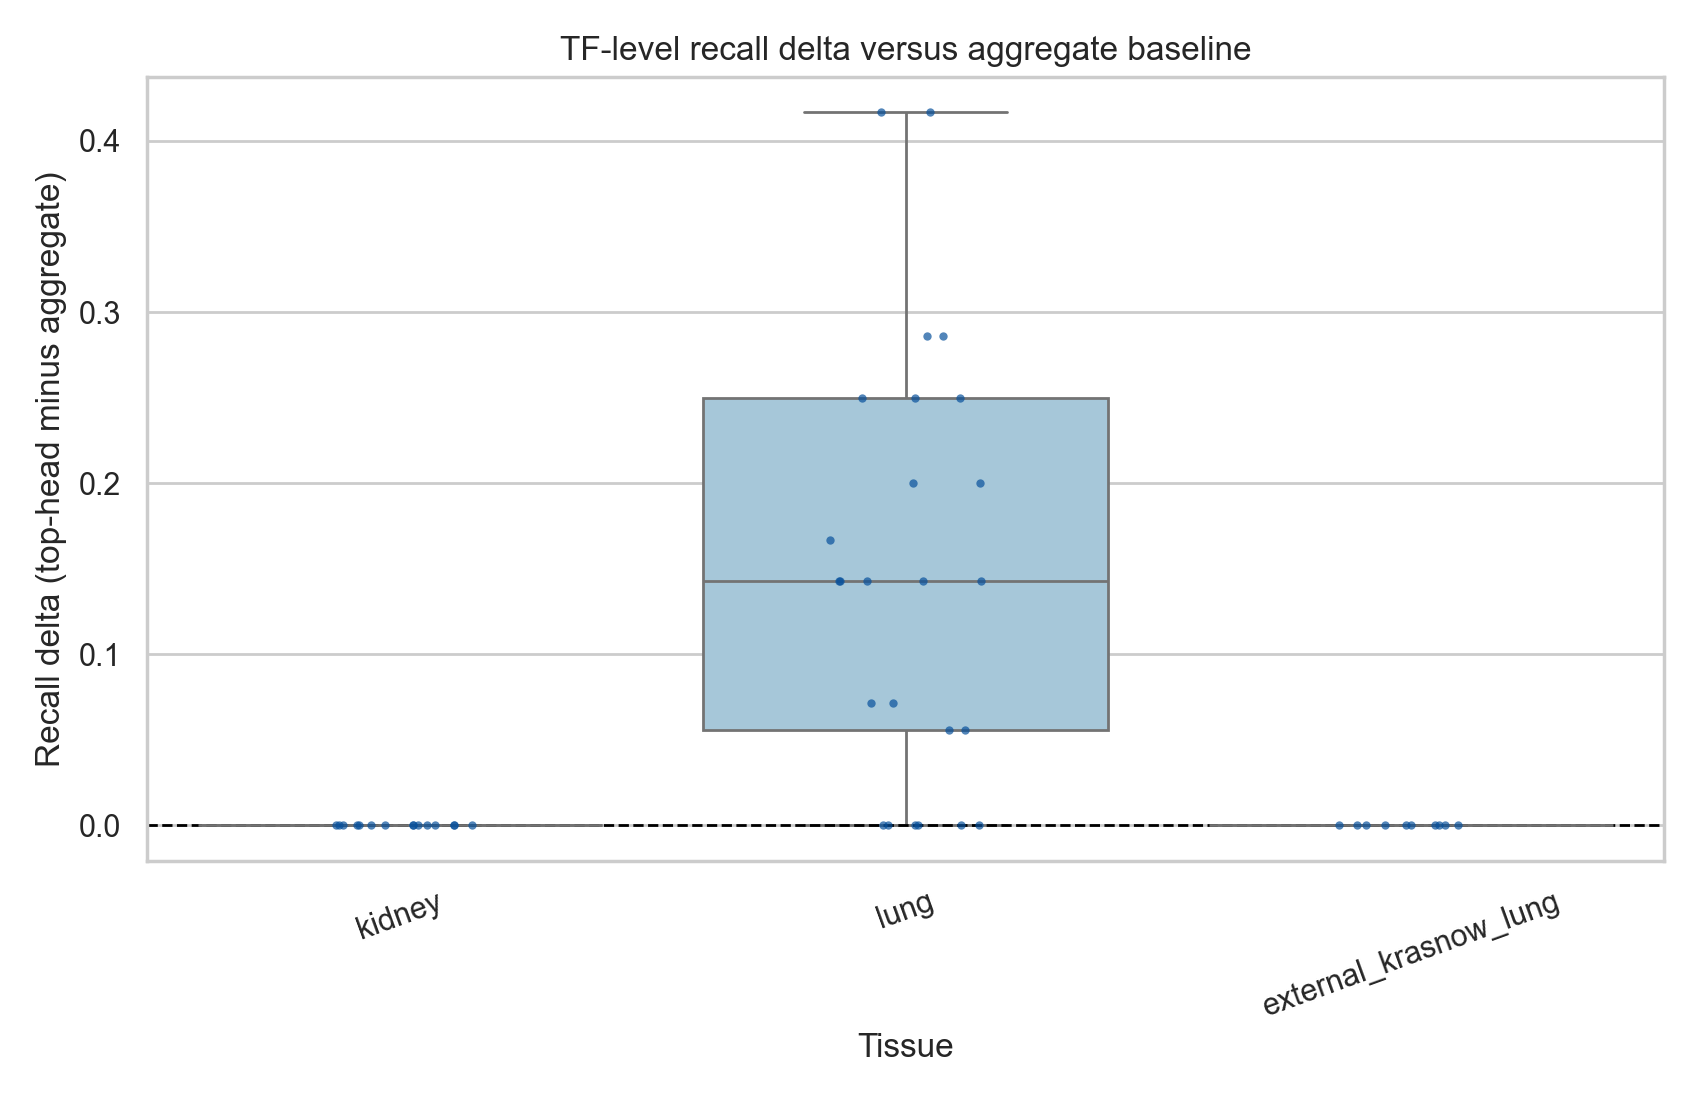
\includegraphics[width=0.48\textwidth]{extended_tf_delta_distribution.png}
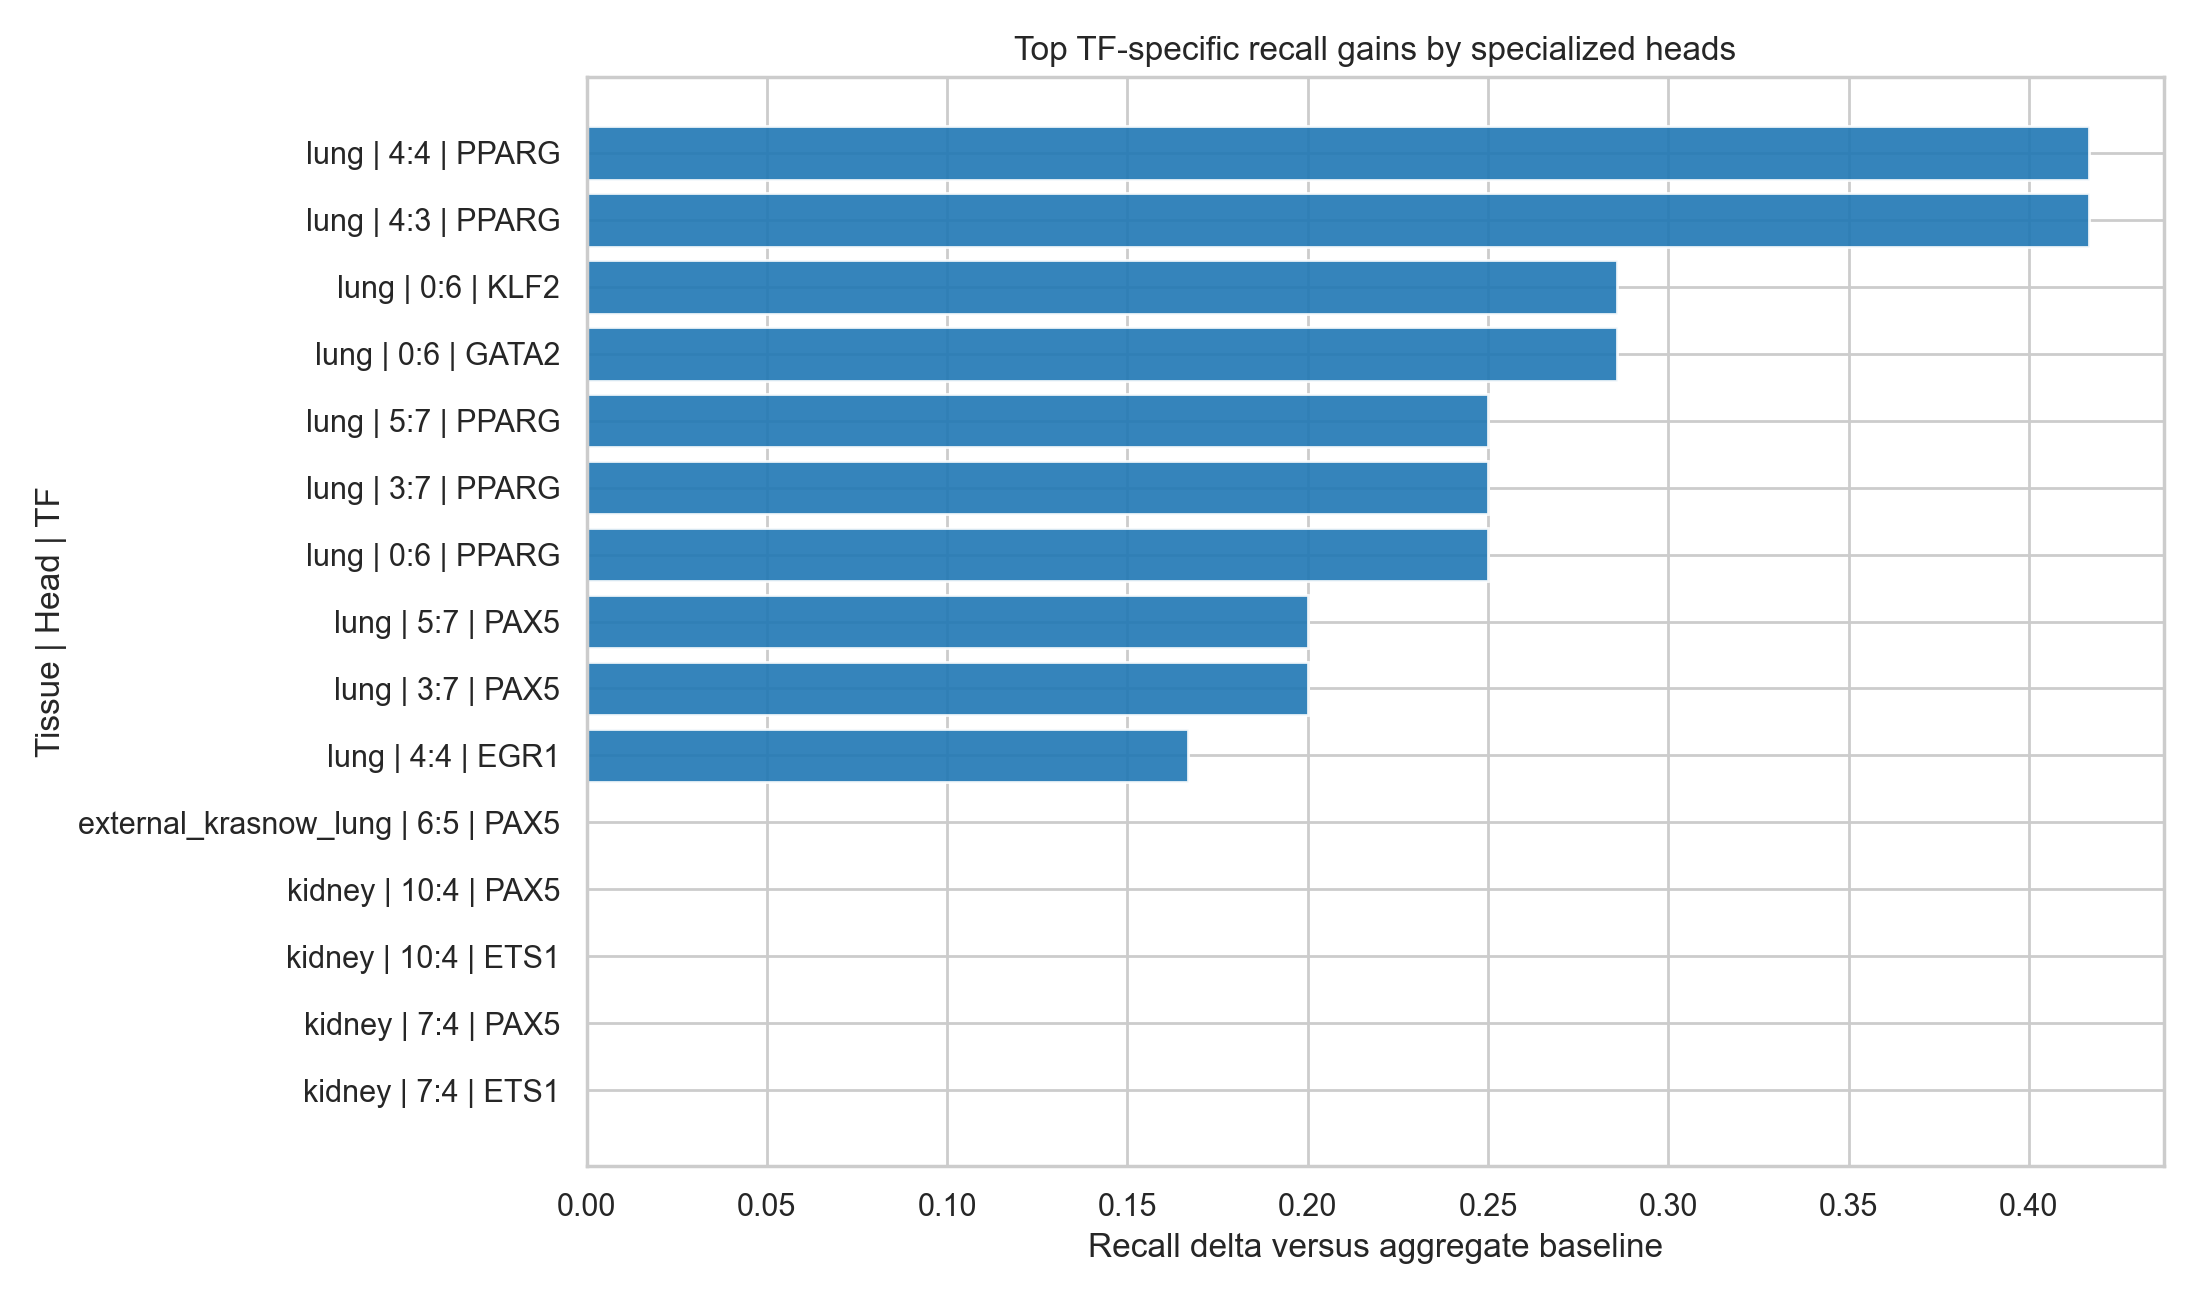
\includegraphics[width=0.48\textwidth]{extended_tf_delta_top.png}
\caption{TF-level head effects. Left: tissue-wise distribution of recall deltas versus aggregate baseline. Right: top tissue/head/TF combinations by positive recall delta.}
\label{fig:tf-delta}
\end{figure}

From the TF tissue-statistics summary:
\begin{itemize}
\item lung: 19/25 TF entries with positive delta, mean delta 0.148, max delta 0.417,
\item kidney: 0/15 positive deltas,
\item external lung: 0/10 positive deltas.
\end{itemize}

Top lung regulator gains are concentrated in specific heads: PPARG reaches +0.417 at heads 4:3 and 4:4, while GATA2 and KLF2 gain +0.286 at head 0:6. This indicates that biologically meaningful head specialization can be sharply tissue-dependent even when global atlas trends are present.

\subsection{Bridge analysis: tissue-top heads versus global evidence heads}
\begin{figure}[H]
\centering
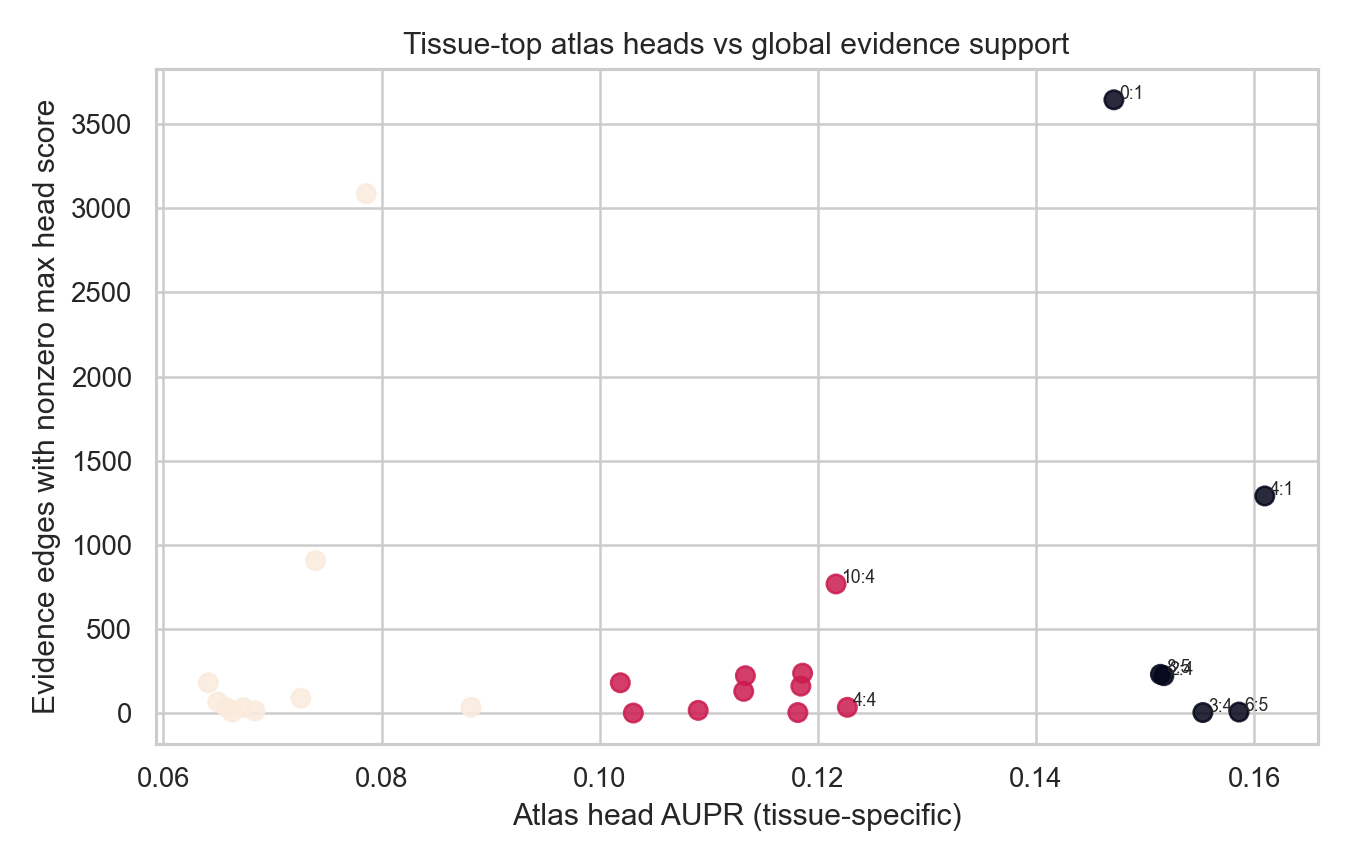
\includegraphics[width=0.8\textwidth]{extended_bridge_scatter.png}
\caption{Tissue-top atlas heads versus global evidence support (nonzero edge counts). High AUPR tissue heads and high-confidence global heads are not the same set in this run.}
\label{fig:bridge-scatter}
\end{figure}

Bridge summary:
\begin{itemize}
\item robust atlas heads (non-immune tissues): 22 unique heads,
\item high-confidence evidence heads: \{0:3, 0:5, 9:1\},
\item set overlap: 0.
\end{itemize}

This implies a two-level functional organization: tissue-optimized ranking heads and reusable biological program heads.

\subsection{Research-grade follow-up experiments}
\paragraph{Checkpoint replication with corrected edge construction.}
The first follow-up experiment reran checkpoint replication after fixing a critical artifact: prior checkpoint edge files carried zero scores and produced non-informative enrichment tests. We rebuilt per-checkpoint inferred edges from nonzero checkpoint attention tensors (TF-source constrained, 1,587 nonzero edges per checkpoint), regenerated edge-level evidence, and repeated threshold-robust enrichment.

\begin{figure}[H]
\centering
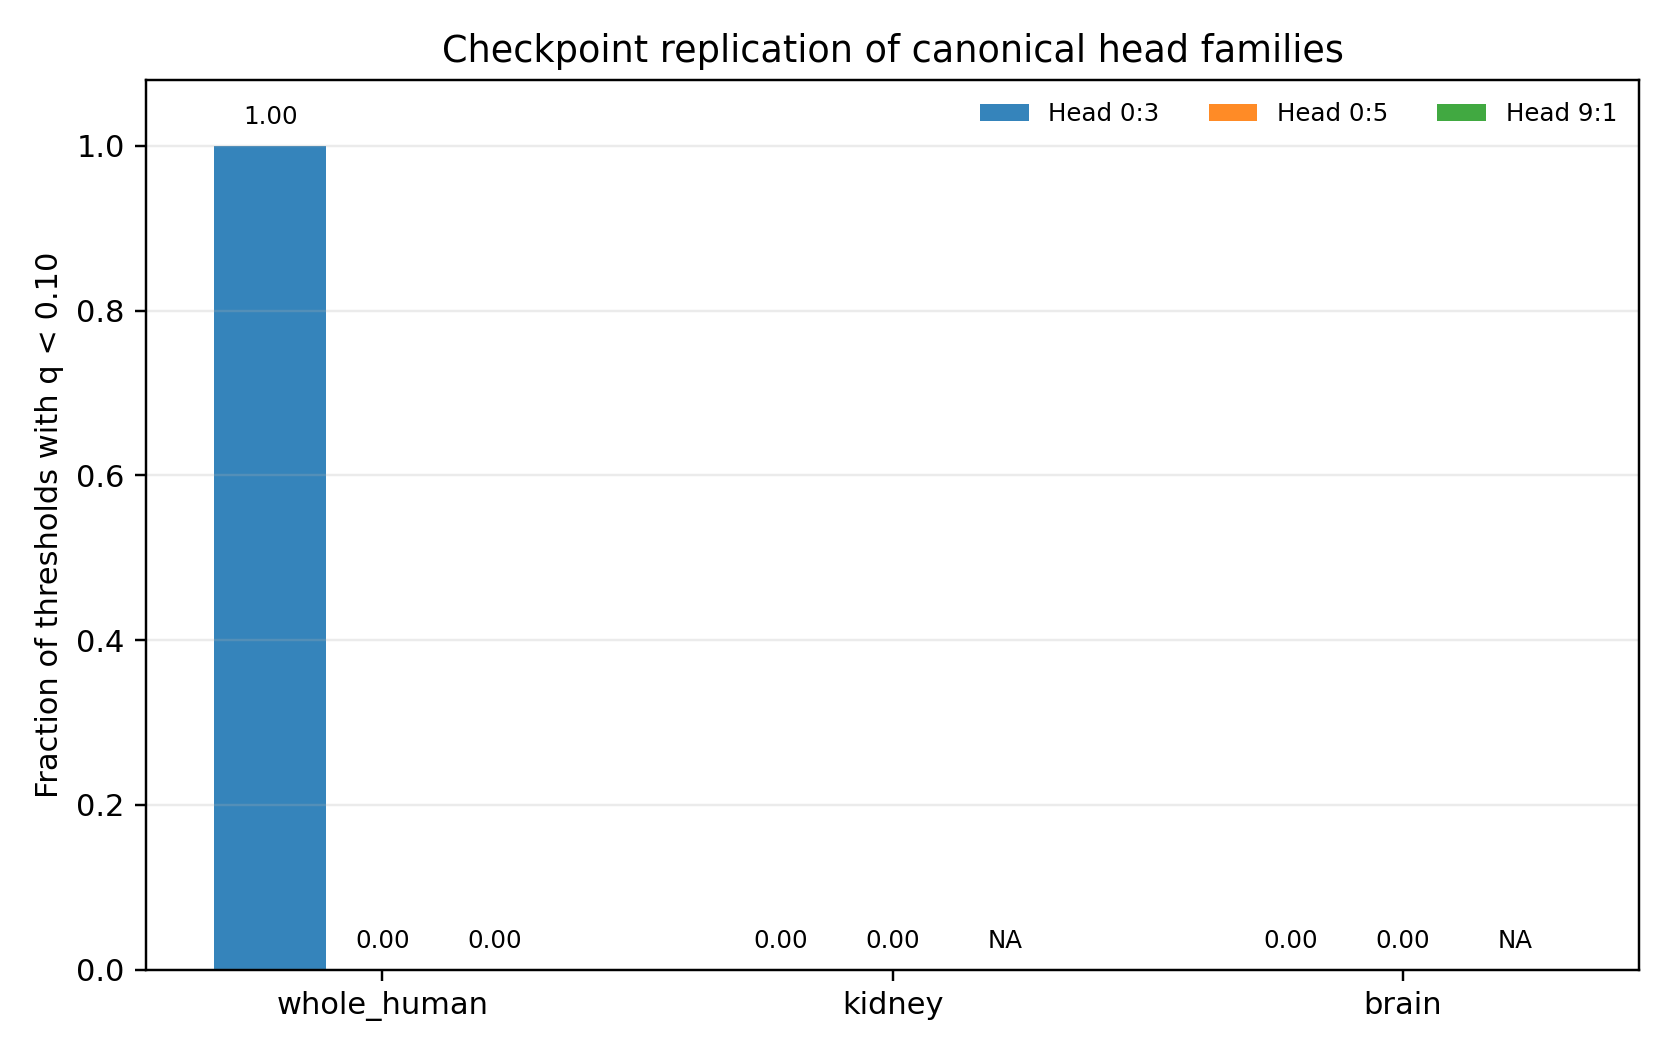
\includegraphics[width=0.75\textwidth]{checkpoint_head_family_replication_bar.png}
\caption{Checkpoint replication of canonical head families as fraction of tested thresholds (top 20/15/10/5\%) with q<0.10.}
\label{fig:checkpoint-replication}
\end{figure}

Canonical-head summary:
\begin{itemize}
\item head 0:3: significant at 4/4 thresholds in whole-human (min q \(1.15\times10^{-14}\)), rank 4 in kidney and rank 5 in brain but not significant there,
\item head 0:5: not significant in these checkpoint tests (0/4 across checkpoints),
\item head 9:1: underpowered in kidney/brain under nonzero-edge count filters.
\end{itemize}

Interpretation: replication is partial but now scientifically meaningful; the strongest prior immune-family head (0:3) survives in at least one independent checkpoint and remains near the top in others.

\paragraph{Immune candidate-space expansion with degeneracy control.}
To move beyond strict-vs-fully-expanded extremes, we added a \texttt{source\_only} candidate regime. This yields a calibrated middle point:
\begin{itemize}
\item strict: 314 candidates, positive rate \(9.55\times10^{-2}\), top-head \(\Delta\)AUPR \(=0.0809\),
\item source-only: 13,189 candidates, positive rate \(2.28\times10^{-3}\), top-head \(\Delta\)AUPR \(=0.00861\),
\item fully expanded: 1,438,800 candidates, positive rate \(2.09\times10^{-5}\), top-head \(\Delta\)AUPR \(=0.00316\).
\end{itemize}

\begin{figure}[H]
\centering
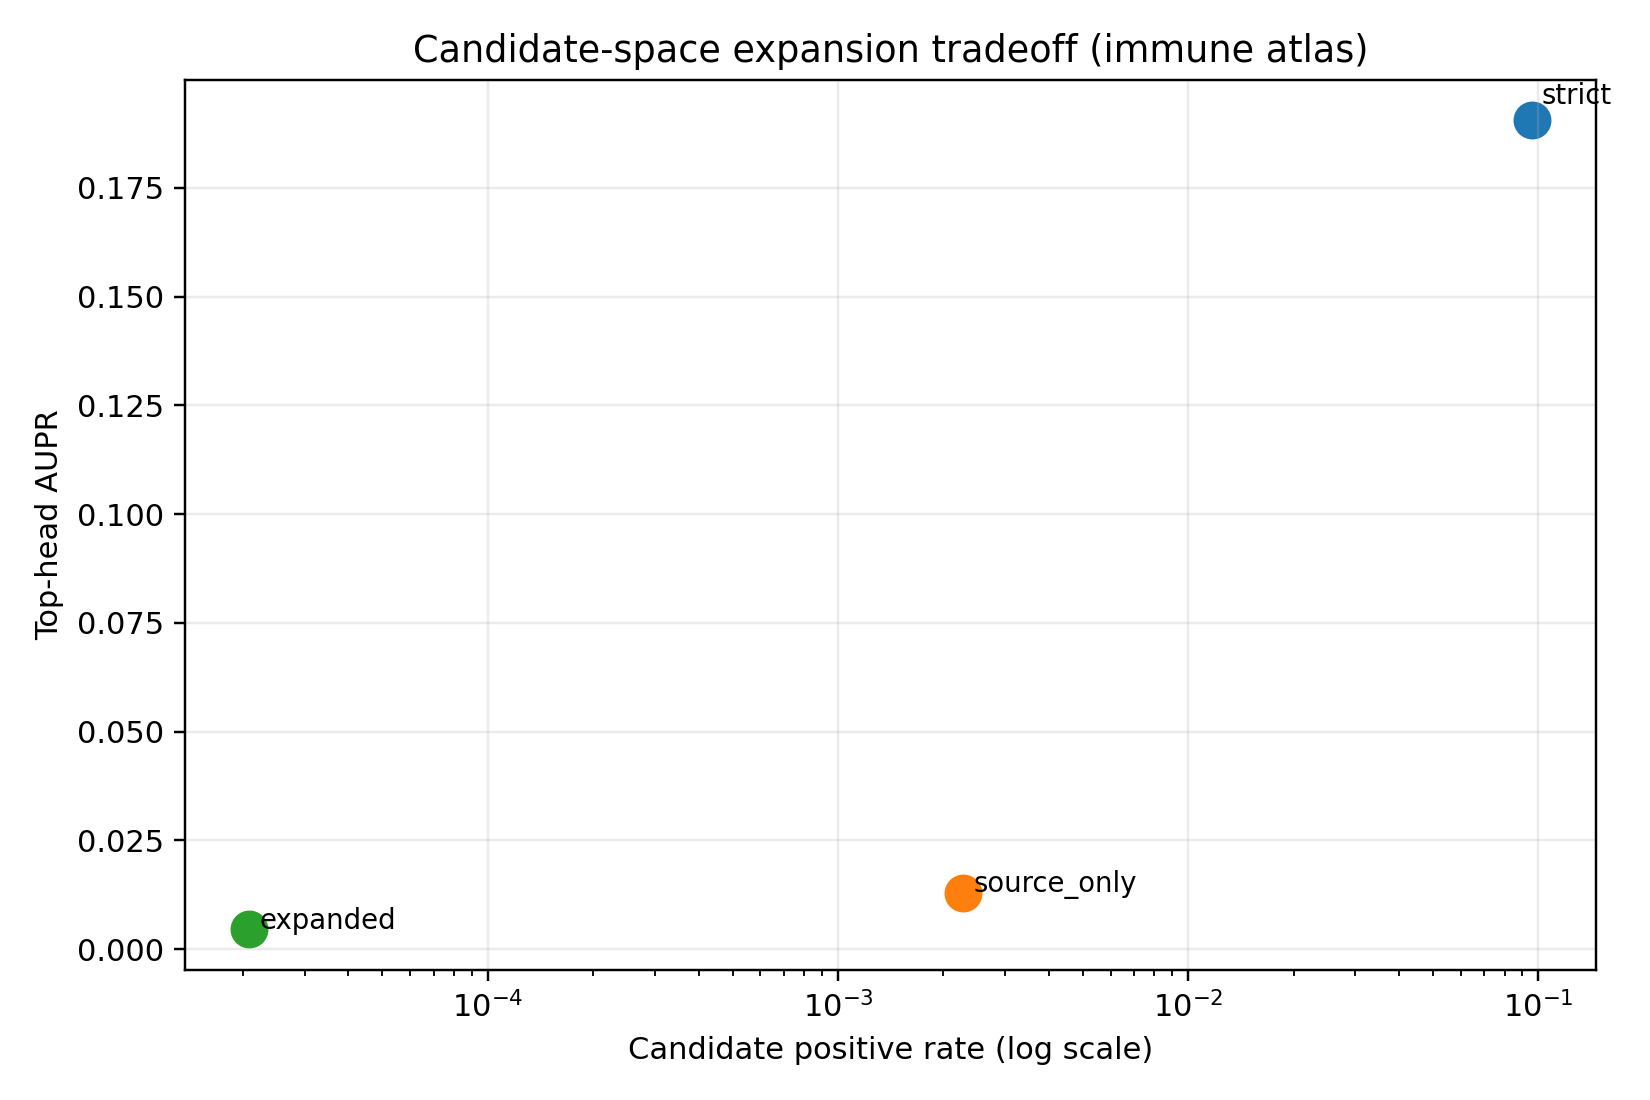
\includegraphics[width=0.72\textwidth]{candidate_space_tradeoff_curve.png}
\caption{Candidate-space tradeoff: as class prior collapses, top-head AUPR drops; source-only masking provides a usable middle regime.}
\label{fig:candidate-tradeoff}
\end{figure}

Interpretation: full expansion remains too imbalanced for stable specialization claims, while source-only masking alleviates strict-space degeneracy without collapsing to the expanded regime.

\paragraph{Targeted causal perturbation validation for immune/metabolic families.}
The initial targeted validation failed with zero-overlap metrics. We replaced it with overlap-aware family manifests:
\begin{itemize}
\item immune family: ETS1/EGR1 overlap pairs evaluated against Dixit 7-day perturbation \cite{dixit2016perturb},
\item metabolic family: CREB1/DDIT3 overlap pairs evaluated against Adamson perturbation \cite{adamson2016multiplexed}.
\end{itemize}
Using top-500 perturbation targets per source (to avoid all-positive labeling), both families yield non-degenerate metrics:
\begin{itemize}
\item immune: \(n_{\text{pairs}}=25\), \(n_{\text{pos}}=9\), AUPR \(=0.434\), AUROC \(=0.583\), permutation \(p=0.150\),
\item metabolic: \(n_{\text{pairs}}=29\), \(n_{\text{pos}}=12\), AUPR \(=0.405\), AUROC \(=0.475\), permutation \(p=0.451\).
\end{itemize}

\begin{figure}[H]
\centering
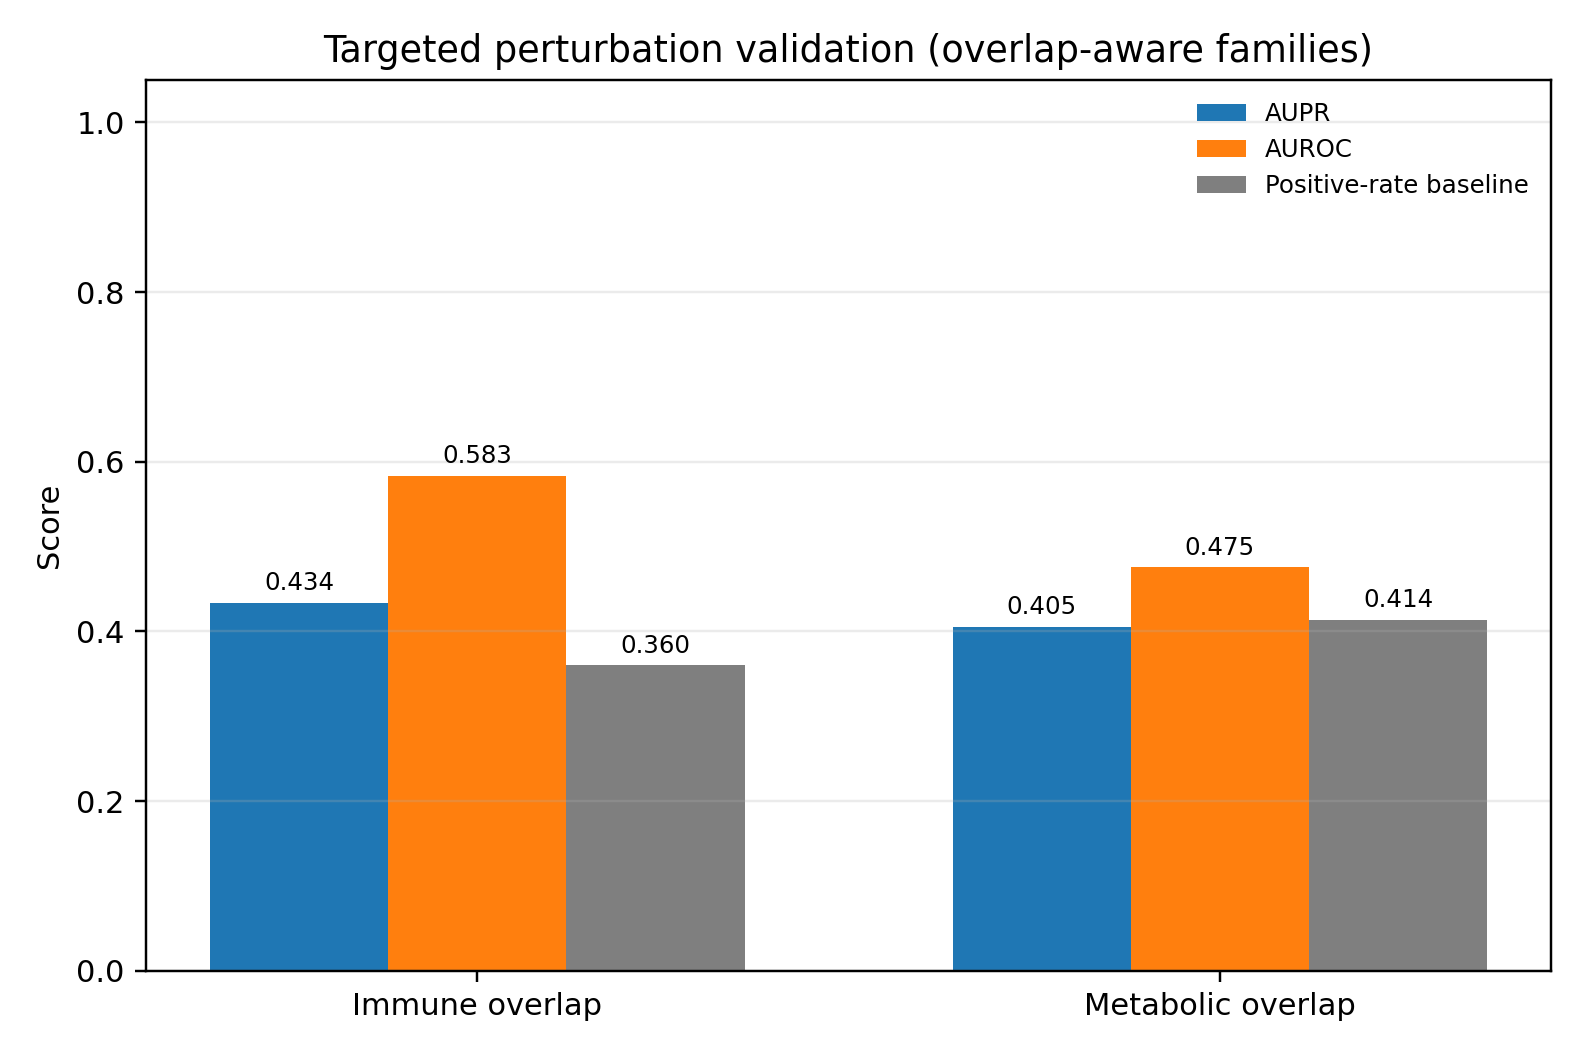
\includegraphics[width=0.75\textwidth]{targeted_perturbation_overlap_metrics.png}
\caption{Overlap-aware targeted perturbation validation for immune and metabolic head families.}
\label{fig:targeted-perturb}
\end{figure}

Interpretation: the causal-to-perturbation bridge is now evaluable and moderate in strength, supporting cautious alignment claims rather than strong causal equivalence.

\section{Discussion}
\subsection{From ``best head'' to head-family ecology}
The expanded results support a head-family view:
\begin{enumerate}
\item \textbf{Fallback sparse heads} (example: 8:0) with high volume but negligible confidence,
\item \textbf{Immune/adaptive heads} (0:3, 0:5, 0:1) enriched for high-confidence edges and immune terms, with 0:3/0:5 stable across all tested confidence thresholds,
\item \textbf{Metabolic head} (9:1) enriched for small-molecule/catabolic programs and stable in 3/4 thresholds,
\item \textbf{Tissue-optimized heads} that maximize per-tissue AUPR but do not necessarily dominate global evidence attribution.
\end{enumerate}

\subsection{Interpretive implications}
This decomposition yields actionable guidance:
\begin{itemize}
\item prioritize immune heads for immune-focused mechanistic hypotheses,
\item prioritize metabolic heads for state/metabolism mechanisms,
\item for lung-specific TF studies, prioritize heads 4:3, 4:4, and 0:6 due to concentrated PPARG/GATA2/KLF2 gains,
\item downweight fallback heads in candidate prioritization workflows.
\end{itemize}

\subsection{What still does not hold}
Despite broader analysis, corrected cross-tissue conservation remains unsupported. The paper therefore emphasizes strong tissue-level and functional-family claims rather than universal conservation.

\section{Limitations}
\begin{itemize}
\item Immune atlas benchmark remains degenerate (\texttt{candidate\_pairs=2}) and should be repaired before strong immune-specific conclusions.
\item Cross-tissue overlap significance does not survive family-wise correction.
\item Current atlas evidence spans a limited checkpoint set and should be expanded before stronger universality claims.
\item GO analysis is enrichment-based and not a causal validation of biological mechanism.
\item TF-level gains are concentrated in lung for this benchmark panel; broader regulator panels are needed before cross-tissue TF generalization.
\end{itemize}

\section{Future Work}
Next highest-value experiments after the present follow-up set:
\begin{enumerate}
\item broaden checkpoint replication beyond three checkpoints and include model-size scaling controls,
\item extend overlap-aware perturbation validation to additional perturbation panels with richer immune TF coverage,
\item test whether source-only candidate masking remains optimal under cross-tissue transfer rather than immune-only benchmarking.
\end{enumerate}

\section{Conclusion}
This full-length analysis upgrades the project from a concise score report to a biologically interpretable mechanistic atlas. We provide robust evidence for tissue specialization, a clear decomposition of head behaviors, and a concrete explanation for why some heads look important but carry little signal. The outcome is a more rigorous and practical foundation for follow-up mechanistic biology work.

\section*{Data and Code Availability}
All code, analysis pipelines, configuration files, and figure-generation scripts are publicly available at \url{[ANONYMOUS REPOSITORY]}. The repository README provides instructions for reproducing all main figures and tables, including supplementary robustness analyses. Dataset-access instructions for Tabula Sapiens and perturbation resources are also provided in the repository documentation.

\begin{thebibliography}{99}
\bibitem{adebayo2018sanity}
Julius Adebayo, Justin Gilmer, Michael Muelly, Ian Goodfellow, Moritz Hardt, and Been Kim.
\newblock Sanity Checks for Saliency Maps.
\newblock In \emph{NeurIPS}, 2018.

\bibitem{adamson2016multiplexed}
Brad Adamson, Thomas Norman, Marco Jost, Min Y. Cho, et al.
\newblock A Multiplexed Single-Cell CRISPR Screening Platform Enables Systematic Dissection of the Unfolded Protein Response.
\newblock \emph{Cell}, 167(7):1867--1882.e21, 2016.

\bibitem{benjamini1995fdr}
Yoav Benjamini and Yosef Hochberg.
\newblock Controlling the False Discovery Rate: A Practical and Powerful Approach to Multiple Testing.
\newblock \emph{Journal of the Royal Statistical Society: Series B}, 57(1):289--300, 1995.

\bibitem{cui2024scgpt}
Haotian Cui, Chloe Wang, Hassaan Maan, et al.
\newblock scGPT: toward building a foundation model for single-cell multi-omics using generative AI.
\newblock \emph{Nature Methods}, 2024.

\bibitem{dixit2016perturb}
Atul Dixit, Oren Parnas, Biyu Li, et al.
\newblock Perturb-Seq: Dissecting Molecular Circuits with Scalable Single-Cell RNA Profiling of Pooled Genetic Screens.
\newblock \emph{Cell}, 167(7):1853--1866.e17, 2016.

\bibitem{elhage2022toy}
Nelson Elhage, Nicholas Schiefer, Aditi Varma, et al.
\newblock Toy Models of Superposition.
\newblock \emph{Transformer Circuits Thread}, 2022.

\bibitem{fisher1922}
R. A. Fisher.
\newblock On the Interpretation of $\chi^2$ from Contingency Tables, and the Calculation of P.
\newblock \emph{Journal of the Royal Statistical Society}, 85(1):87--94, 1922.

\bibitem{geiger2021causal}
Atticus Geiger, Hanson Lu, Thomas Icard, and Christopher Potts.
\newblock Causal Abstractions of Neural Networks.
\newblock In \emph{NeurIPS}, 2021.

\bibitem{han2018trrust}
Hyeshik Han, Jae-Won Cho, Sangyoung Lee, et al.
\newblock TRRUST v2: an expanded reference database of human and mouse transcriptional regulatory interactions.
\newblock \emph{Nucleic Acids Research}, 46(D1):D380--D386, 2018.

\bibitem{hao2024scfoundation}
Mingyao Hao, Jiarui Li, Hongwei Li, et al.
\newblock Towards foundation models for single-cell biology.
\newblock \emph{Nature Methods}, 2024.

\bibitem{jain2019attention}
Sarthak Jain and Byron C. Wallace.
\newblock Attention is not Explanation.
\newblock In \emph{NAACL}, 2019.

\bibitem{jones2022tabula}
R. C. Jones, M. Karkanias, M. A. Krasnow, et al.
\newblock The Tabula Sapiens: A multiple-organ, single-cell transcriptomic atlas of humans.
\newblock \emph{Science}, 376(6594):eabl4896, 2022.

\bibitem{kolberg2020gprofiler2}
Liis Kolberg, Uku Raudvere, Ivan Kuzmin, et al.
\newblock gprofiler2 -- an R package for gene list functional enrichment analysis and namespace conversion toolset.
\newblock \emph{F1000Research}, 9:ELIXIR-709, 2020.

\bibitem{olah2020zoom}
Chris Olah, Nick Cammarata, Ludwig Schubert, et al.
\newblock Zoom In: An Introduction to Circuits.
\newblock \emph{Distill}, 2020.

\bibitem{theodoris2023geneformer}
Christos V. Theodoris, Linghao Xiao, Aaron Chopra, et al.
\newblock Transfer learning enables predictions in network biology.
\newblock \emph{Nature}, 618:616--624, 2023.

\bibitem{vig2020causal}
Jesse Vig, Yonatan Belinkov, Siddharth Jayakumar, et al.
\newblock Causal Mediation Analysis for Interpreting Neural NLP: The Case of Gender Bias.
\newblock \emph{Transactions of the ACL}, 8:7--20, 2020.
\end{thebibliography}

\end{document}
